\documentclass[a4paper]{article}
\usepackage[left=2cm,right=2cm,
    top=2cm,bottom=2cm,bindingoffset=0cm]{geometry}
\usepackage[T2A]{fontenc}
\usepackage[utf8]{inputenc}
\usepackage[english,russian]{babel}
\usepackage{indentfirst}
\usepackage[final]{graphicx}
\usepackage{algorithm}
\usepackage{algorithmic}
\usepackage{multirow}
\usepackage{longtable}
\usepackage{tabulary}
\usepackage{placeins}
\usepackage{needspace}
\usepackage{color}

\usepackage{listings}

%\usepackage{hyperref}
%\hypersetup{
%    colorlinks=black,
    %citecolor=black,
   % filecolor=black,
  %  linkcolor=black,
 %   urlcolor=black
%}


\graphicspath{{Images/}}
\DeclareGraphicsExtensions{.pdf,.png,.jpg,.svg}

\renewcommand{\labelenumi}{\arabic{enumi}.}
\renewcommand{\labelenumii}{\asbuk{enumii})}


\author{Пахтусов Н. Г., ПРО-306}
\makeatletter
\begin{document}

\begin{center}
\thispagestyle{empty} 

Федеральное государственное бюджетное образовательное учереждение высшего \\
профессионального образования\\
<<Уфимский государственный авиационный технический университет>>
\vspace*{\fill}
\begingroup
\centering

Отчёт по лабораторной работе\\
по дисциплине: <<Архитектура вычислительных систем>>\\
<<Основы работы с Internet (комплексом протоколов TCP/IP)>>

\endgroup
\vspace*{\fill}

\end{center}

\begin{flushright}

Выполнил:\\
\@author \\
Проверил: \\
Верхотуров М. А.

\end{flushright}

\begin{center}
Уфа, 2015
\end{center}

\clearpage
\tableofcontents
\clearpage

\section{Цель работы и постановка задачи}
\textbf{Цель работы:} Получение навыков установки и конфигурации стека протоколов TCP/IP, определение работоспособности интересующего узла или канала связи, изучение основ организациибезопасной работы в Internet.

\textbf{Постановка задачи:} Установка и конфигурирование стека протоколов TCP/IP. Обследование локальной, кафедральной и университетской сетей; установка и конфигурирование и работа с межсетевым экраном (<<Firewall>>).

\textbf{Формальная постановка задачи}

\begin{figure}[H]
	\center{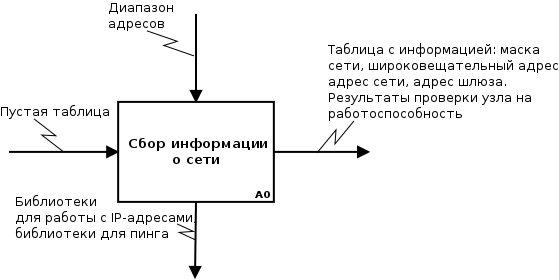
\includegraphics[width = 0.9\linewidth]{image0}}
			\caption{Формальная постановка задачи}
\end{figure}

\section{Структура решения задачи (этапы решения)}

\begin{enumerate}
	\item Описание TCP/IP-параметров настройки компьютера.
	\begin{enumerate}
		\item Настройка параметров.
		\item Просмотр параметров.
	\end{enumerate}
	\item Структура локальной (кафедральной), факультетской и университетской сетей с указанием IP и доменных адресов.
		\begin{enumerate}
		\item Сбор информации о сети. Определение работоспособности каждого узла и его символьного (доменного) имени.
		\item Анализ сети. Определение следующих параметров: адрес сети, адрес шлюза, маска, широковещательный адрес.
		\item Построение карты сети.
	\end{enumerate}
	\item Параметры настройки Firewall
		\begin{enumerate}
		\item Установка Firewall
		\item Конфигурирование Firewall
	\end{enumerate}
\end{enumerate}

\section{Теория}
Каждый компьютер в сети TCP/IP имеет адреа трёх уровней:

\textbf{MAC-адрес} -- локальный адрес узла или физический адрес для узлов, входящих в локальную сеть. Эти адреса назначаются производителями сетевого оборудования и являются уникальными. MAC-адрес состоит из 6 байтов: старшие 3 байта -- идентификатор фирмы-производителя, а младшие 3 назаначаются уникальным образом своим производителем. Для узлов, входящих в глобальные сети, такие, как Х.25 или frame relay, локальный адрес назначается администратором глобальной сети.

\textbf{IP-адрес} -- уникальный адрес, назначающийся каждому узлу сети TCP/IP, который используется во всех сеансах связи с этим узлом. В зависимости от версии протокола IP, он может быть 32х-разрядным (IPv4) или 128 разрядным (IPv6). Он назначается администратором. По протоколу IPv4 IP-адрес состоит из двух частей: номера сети и номера узла. Для внутренних сетей номер сети может быть быть выбран произвольно. Для сетей, подключённых к Internet, номер сети назначается по рекомендации организации по назначению имен и адресов в Interet (ICANN).

Номер узла в протоколе IP назначается независимо от физического адреса узла. Деление IP-адреса на поле номера сети и номера узла -- гибкое, и граница между этими полями может устонавливаться весьма произвольно. Узел может входить в несколько IP-сетей. В этом случае узел должен иметь несколько IP-адресов (по числу сетевых связей). Таким образом, IP-адрес характеризует не отдельный узел, а одно сетевое соединение.

\textbf{DNS-имя} -- символьный идентификатор-имя, например, \emph{proxy.ugatu.net}. Этот адрес назначается администратором и состоит из нескольких частей, например, имени машины, имени организации, имени домена. Используется на прикладном уровне, например, в протоколах FTP или TelNET.

\subsection{Протокол IP}

	\subsubsection{IPv4}

		\textbf{Классы IP-адресов протокола IPv4}.

		Разбивая IP-адреса на пару значений, первое из которых характеризует сеть, а второе -- узел, получаем 4 разных класса IP адресов:
		\begin{itemize}

			\item
				\textbf{Класс А}:\\
				Адреса класса А назначаются узлам очень большой сети. Старший бит в адресах этого класса -- всегда 0. Следующие 7 бит представляют собой идентификатор сети. Оставшиеся 24 -- содержат идентификатор узла. Это позволяет иметь 126 сетей -- и до 17 миллионов в каждой.
			\item
				\textbf{Класс В}:\\
				Адреса класса В назначаются узлам в больших и средних по размеру сетях. В двух старших битах IP-адреса класса B записывается 1 0. Следующие 14 бит содержат идентификатор сети. Оставшиеся 16 бит представляют идентификатор узла, и таким образом, возможно существование 16'384 сетей класса В, в каждой из которых возможно около 65'000 узлов.
			\item
				\textbf{Класс С}:\\
				Адреса класса С применяются в небольших сетях. Три старших бита IP-адреса этого класса содержат двоичное значение 1 1 0. Следующие 21 бит составляет идентификатор сети, а оставшиеся 8 отводятся под идентификатор узла. Всего возможно около 2'000'000 сетей класса С, содержащих каждая 254 узла.
			\item
				\textbf{Класс D}. Адреса класса D обозначают особый, групповой адрес -- multicast. Если в пакете в качестве адреса назначения указан адрес класса D, то такой пакет должны получить все узлы, которым присвоен данный адрес. Адреса класса D начинаются с последовательности 1110.

			\item
				\textbf{Класс Е}. Адреса класса E начинаются с последовательности 11110. Это экспериментальный класс и он зарезервирован для будущих применений.

		\end{itemize}

В таблице приведены диапазоны номеров сетей, соответствующих каждому классу сетей.

		\begin{center}
			\begin{tabular}{|c|c|c|}
			\hline
			Класс&Наименьший адрес&Наибольший адрес\\
			\hline
			A&1.0.0.0&126.0.0.0\\
			B&128.0.0.0&191.255.0.0\\
			C&192.0.1.0.&223.255.255.0\\
			D&224.0.0.0&239.255.255.255\\
			E&240.0.0.0&247.255.255.255\\
			\hline
		\end{tabular}
	\end{center}

		\textbf{Широковещательный адрес} -- условный (не присвоенный никакому устройству в сети) адрес, который используется для широковещательного режима передачи, при котором пакеты передаются сразу всем компьютерам конкретной сети. Широковещательный адрес -- последний адрес в диапозоне, задаваемый маской.

		\textbf{Маска сети} -- битовая маска, определяющая, какая часть IP-адреса узла сети отностися к адресу сети, а какая -- к адресу самого узла этой сети. Например, узел с IP-адресом 12.34.56.78 и маской подсети 255.255.255.0 находится в сети 12.34.56.0/24, где 24 -- длина префикса в битах.

		\textbf{CIDR.}

		\textbf{Бесклассовая адресация} (\emph{Classless Inter-Domain Routing}) -- метод IP-адресации, позволяющий гибко управлять пространством IP-адресов, не используя жёсткие рамки классовой адресации. Использование этого метода позволяет экономно использовать ограниченный ресурс IP-адресов, поскольку возможно применение различных масок подсетей к различным подсетям. Бесклассовая авторизация основывается на переменной длине маски подсети. Длина префикса сети передаётся вместе с адресом, например, 192.233.147.200/27. Таким образом, указывается, что 27 бит отводится под префикс сети, а оставшиеся 5 бит -- указывают адрес компьютера в сети.
		
	\subsubsection{IPv6}
		IPv6 — новая версия протокола IP, призванная решить проблемы, с которыми столкнулась предыдущая версия (IPv4) при её использовании в Интернете, за счёт использования длины адреса 128 бит вместо 32.
		
		В IPv6 адрес представляется в виде последовательности 16-битных чисел, представленных в шеснадцатиричной системе исчисления и разделённых двоеточием, например,\\ C8E6:8C64:FFFF:FFFF:0:1180:96A:FFFF.\\
		Ряд повторяющихся нулей может быть заменён парой двоеточий:\\
		FF05:0:0:0:0:0:0:1180:96A
		
		Так же как и в четвертой версии протокола в шестой версии адрес соответствует соединению, а не компьютеру.
		
		В IPv6 сохраняется (и расширяется) иерархия адресов IPv4. Однако, чтобы сделать распределение и изменение адресов более простым, в протоколе IPv6 можно назначить для одной сети несколько префиксов, а один компьютер может иметь несколько различных адресов, соответствующих одному и тому же соединению.
		
\subsection{Подсети}

	Важным элементом разбиения адресного пространства Internet являются подсети. \textbf{Подсеть} -- это подмножество сети, не пересекающееся с другими подсетями. Это означает, что сеть организации может быть разбита на фрагменты, каждый из которых будет составлять подсеть. Реально, каждая подсеть соответствует физической локальной сети (например, сегменту Ethernet). Подсети придуманы для того, чтобы обойти ограничения физических сетей на число узлов в них и максимальную длину кабеля в сегменте сети. Например, сегмент тонкого Ethernet имеет максимальную длину 185м и может включать до 32 узлов. Самая маленькая сеть -- класса С -- может состоять из 254 узлов. Для того чтобы достичь этой цифры, надо объединить несколько физических сегментов сети. Сделать это можно либо с помощью физических устройств (например, репитеров), либо при помощи маршрутизаторов. \textbf{Маршрутизатор} -- специализированный сетевой компьютер, имеющий минимум два сетевых интерфейса и пересылающий пакеты данных между различными сегментами сети, принимающий решения о пересылке на основании информации о топологии сети и определённых правил, заданных администратором.

	На рисунке \ref{fig:addresSceme} изображен фрагмент сети класса B -- 144.206.0.0, состоящий из двух подсетей -- 144.206.130.0 и 144.206.160.0. В центре схемы изображена машина шлюз, которая связывает подсети. Эта машина имеет два сетевых интерфейса и, соответственно, два IP-адреса.

	\begin{figure}[h]
		\center{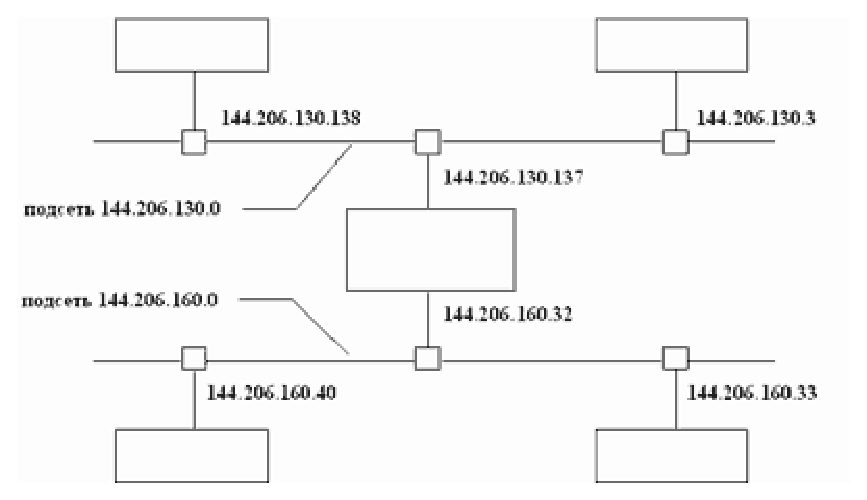
\includegraphics[width=0.5\linewidth]{intsr_19}}
		\caption{Схема разбиения адресного пространства сети на подсети}
		\label{fig:addresSceme}
	\end{figure}

	В принципе, разбивать сеть на подсети необязательно. Можно использовать адреса сетей другого 
класса (с меньшим максимальным количеством узлов). Но при этом возникает, как минимум, два 
неудобства:

	Во-первых, в сети, состоящей из одного сегмента Ethernet, весь адресный пул сети не будет использован, так как, например, для сети класса С (самой маленькой с точки зрения количества узлов в ней), из 254 возможных адресов можно использовать только 32.

	Во-вторых, все машины за пределами организации, которым разрешен доступ к компьютерам сети данной организации, должны знать шлюзы для каждой из сетей. Структура сети становится открытой во внешний мир. Любые изменения структуры могут вызвать ошибки маршрутизации. При использовании подсетей внешним машинам надо знать только шлюз всей сети организации. Маршрутизация внутри сети -- это ее внутреннее дело.

	Разбиение сети на подсети использует ту часть IP-адреса, которая закреплена за номерами хостов. 
Администратор сети может замаскировать часть IP-адреса и использовать ее для назначения номеров 
подсетей. Фактически, способ разбиения адреса на две части, теперь будет применятся к адресу хоста 
из IP-адреса сети, в которой организуется разбиение на подсети.

	Маска подсети -- это четыре байта, которые накладываются на IP-адрес для получения номера 
подсети. Например, маска 255.255.255.0 позволяет разбить сеть класса В на 254 подсети по 254 узла 
в каждой. На рисунке 2 приведено маскирование подсети 144.206.160.0 из предыдущего примера.

	\begin{figure}[h]
		\center{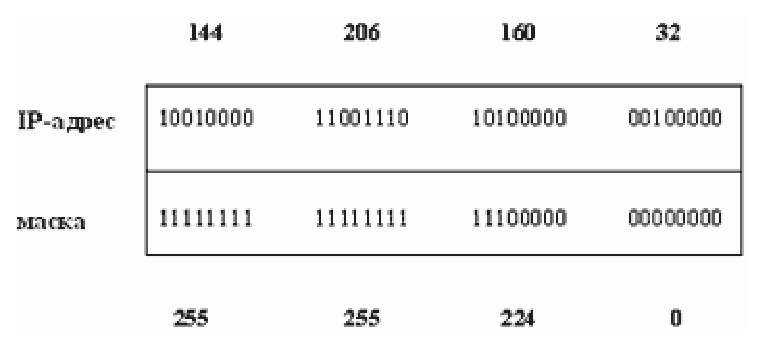
\includegraphics[width=0.5\linewidth]{intsr_20}}
		\caption{Схема маскирования и вычисления номера подсети}
		\label{fig:markSceme}
	\end{figure}
	
	На приведенной схеме (Рис. \ref{fig:markSceme}) сеть класса B (номер начинается с 10) разбивается на подсети маской 255.255.224.0. При этом первые два байта задают адрес сети и не участвуют в разбиении на подсети. Номер подсети задается тремя старшими битами третьего байта маски. Такая маска позволяет получить 6 подсетей. Для нумерации подсети нельзя использовать номер 000 и номер 111. Номер 160 задает 5-ю подсеть в сети 144.206.0.0. Для нумерования машин в подсети можно использовать оставшиеся после маскирования 13 битов, что позволяет создать подсеть из 8190 узлов. Перестроить сеть, состоящую из более чем 400 машин, не такая простая задача, так как ей управляет 4 администратора, которые должны изменить маски на всех машинах сети. Ряд компьютеров работает в круглосуточном режиме и все изменения надо произвести в тот момент, когда это минимально скажется на работе пользователей сети. Данный пример показывает насколько внимательно следует подходить к вопросам планирования архитектуры сети и ее разбиения на подсети. Многие проблемы можно решить за счет аппаратных средств построения сети.

	К сожалению, подсети не только решают, но также и создают ряд проблем. Например, происходит потеря адресов, но уже не по причине физических ограничений, а по причине принципа построения адресов подсети. Как было видно из примера, выделение трех битов на адрес подсети не приводит к образованию 8-ми подсетей. Подсетей образуется только 6, так как номера сетей 0 и 7 использовать в силу специального значения IP-адресов, состоящих из 0 и единиц, нельзя. Таким образом, все комбинации адресов хоста внутри подсети, которые можно было бы связать с этими номерами, придется забыть. Чем шире маска подсети (чем больше места отводится на адрес хоста), тем больше потерь. В ряде случаев приходится выбирать между приобретением еще одной сети или изменением маски. При этом физические ограничения могут быть превышены за счет репитеров, хабов и т. п.	
	
	\subsection{Преобразования адресов для протокола IP}
\begin{figure}[h]
    \centering
    \resizebox{.5\linewidth}{!}{\input{Images/dns.pdf_tex}}
    \caption{Структура DNS}
\end{figure}

	DNS -- это распределённая база данных, поддерживающая иерархическую систему имён для идентификации в сети интернет. Служба DNS предназначена для автоматического поиска IP-адреса по известному символьному имени узла. DNS требует статической конфигурации своих таблиц, отображающих имена компьютеров в IР-адрес.
	
	Протокол DNS является служебным протоколом прикладного уровня. Этот протокол несимметричен -- в нем определены DNS-серверы и DNS-клиенты. DNS-серверы хранят часть распределенной базы данных о соответствии символьных имен и IP-адресов. Эта база данных распределена по административным доменам сети Internet. Клиенты сервера DNS знают IP-адрес сервера DNS своего административного домена и по протоколу IP передают запрос, в котором сообщают известное символьное имя и просят вернуть соответствующий ему ШР-адрес.
	
	Если данные о запрошенном соответствии хранятся в базе данного DNS-сервера, то он сразу посылает ответ клиенту, если же нет -- то он посылает запрос DNS-серверу другого домена, который может сам обработать запрос, либо передать его другому DNS-серверу. Все DNS-серверы соединены иерархически, в соответствии с иерархией доменов сети Internet. Клиент опрашивает эти серверы имен, пока не найдет нужные отображения. Этот процесс ускоряется из-за того, что серверы имен постоянно кэшируют информацию, предоставляемую по запросам. Клиентские компьютеры могут использовать в своей работе IP-адреса нескольких DNS-серверов, для повышения надежности своей работы.
	
	База данных DNS имеет структуру дерева, называемого доменным пространством имен, в котором каждый домен (узел дерева) имеет имя и может содержать поддомены. Имя домена идентифицирует его положение в этой базе данных по отношению к родительскому домену, причем точки в имени отделяют части, соответствующие узлам домена.
	
	Корень базы данных DNS управляется центром Internet Network Information Centre. Домены верхнего уровня назначаются для каждой страны, а также на организационной основе. Имена этих доменов должны следовать международному стандарту ISO 3166. Для обозначения стран используются трехбуквенные и двухбуквенные аббревиатуры, а для различных типов организаций используются следующие аббревиатуры: 
	
	\begin{itemize}
		\item \textbf{соm} -- коммерческие организации (например, microsoft.com).
		\item \textbf{edu} -- образовательные (например, mit.edu).
		\item \textbf{gov} -- правительственные организации (например, nsf.gov).
		\item \textbf{org} -- некоммерческие организации (например, linux.org).
		\item \textbf{net} -- организации, поддерживающие сети (например, nsf.net).
		\item \textbf{io} -- изначально использовался для Британских территорий в Индийском океане, но сейчас используется, в основном, организациями, связанными с компьютерными технологиями.
	\end{itemize}
	
	Каждый домен DNS администрируется отдельной организацией, которая обычно разбивает свой домен на поддомены и передает функции администрирования этих поддоменов другим организациям. Каждый домен имеет уникальное имя, а каждый из поддоменов имеет уникальное имя внутри своего домена. Имя домена может содержать до 63 символов. Каждый хост в сети Internet однозначно определяется своим полным доменным именем (fully qualified domain name, FQDN), которое включает имена всех доменов по направлению от хоста к корню. Пример полного DNS-имени: vmk.ugatu.ac.ru.
	
		\textbf{ARP} (англ. Address Resolution Protocol — протокол определения адреса) --- низкоуровневый протокол, предназначенный для определения МАС-адреса по известному IP-адресу. Как только узлу сети А требуется преобразовать IP-адрес I$_b$, он посылает в режиме широковещания специальный пакет, который предписывает узлу с IP-адресом I$_b$ сообщить свой физический адрес (P$_b$). Данный пакет будет получен всеми узлами сети, включая В. Ответ посылает только узел В, поскольку только ему назначен IP-адрес I$_b$. Получив ответный пакет, узел А использует присланный ему физический адрес для отправки пакетов узлу В. Наибольшее распространение этот протокол получил благодаря повсеместности сетей IP, построенных поверх Ethernet, поскольку практически ввсегда при таком сочетании используется ARP.
		
		\textbf{RARP} (англ. Reverse Address Resolution Protocol) -- обратный протокол преобразования адресов) -- преобразует физический адрес в IP-адрес .Протокол применяется во время загрузки узла, когда он посылает групповое сообщение-запрос со своим физическим адресом. Сервер принимает это сообщение и просматривает свои таблицы (либо перенаправляет запрос куда-либо ещё) в поисках соответствующего физическому, IP-адреса. После обнаружения найденный адрес отсылается обратно на запросивший его узел. Другие станции также могут <<слышать>> этот диалог и локально сохранить эту информацию в своих ARP-таблицах. RARP является дополнением к ARP.
		
	\subsection{Сетевые протоколы}
		\subsubsection{DHCP}
			\textbf{DHCP} (англ. Dynamic Host Configuration Protocol -- протокол динамической настройки узла) -- сетевой протокол, позволяющий компьютерам автоматически получать IP-адрес и другие параметры, необходимые для работы в сети TCP/IP. Данный протокол работает по модели «клиент-сервер». Для автоматической конфигурации компьютер-клиент на этапе конфигурации сетевого устройства обращается к так называемому серверу DHCP, и получает от него нужные параметры. Протокол DHCP предоставляет три способа распределения IP-адресов:
			\begin{itemize}
				\item 
					\textbf{Ручное распределение.} При этом способе сетевой администратор сопоставляет аппаратному адресу (для Ethernet сетей это МАС-адрес) каждого клиентского компьютера определённый IР-адрес. Фактически, данный способ распределения адресов отличается от ручной настройки каждого компьютера лишь тем, что сведения об адресах хранятся централизованно (на сервере DHCP), и потому их проще изменять при необходимости.
				\item 
					\textbf{Автоматическое распределение.} При данном способе каждому компьютеру на постоянное использование выделяется произвольный свободный IP-адрес из определённого администратором диапазона.
				\item 
					\textbf{Динамическое распределение.} Этот способ аналогичен автоматическому распределению, за исключением того, что адрес выдаётся компьютеру не на постоянное пользование, а на определённый срок. Это называется \emph{арендой адреса}. По истечении срока аренды IP-адрес вновь считается свободным, и клиент обязан запросить новый (он, впрочем, может оказаться тем же самым). Кроме того, клиент сам может отказаться от полученного адреса. 
			\end{itemize}
		\subsubsection{ICMP}
			\textbf{ICMP} (англ. Internet Control Message Protocol протокол межсетевых управляющих сообщений) — сетевой протокол, входящий в стек протоколов TCP/IP. В основном ICMP используется для передачи сообщений об ошибках и других исключительных ситуациях, возникших при передаче данных, например, запрашиваемая услуга недоступна, или хост, или маршрутизатор не отвечают. Также на ICMP возлагаются некоторые сервисные функции.
			ICMP основан на протоколе IP. Каждое ICMP-сообщение инкапсулируется непосредственно в пределах одного IP-пакета, и, таким образом, как и UDP и в отличие от TCP, ICMP является т. н. «ненадежным» (не контролирующим доставку и её правильность). В отличие от UDP, где реализация надёжности возложена на ПО прикладного уровня, ICMP (в силу специфики применения) обычно не нуждается в реализации надёжной доставки. Его цели отличны от целей транспортных протоколов, таких как TCP и UDP: он, как правило, не используется для передачи и приёма данных между конечными системами. ICMP не используется непосредственно в приложениях пользователей сети (исключение составляют инструменты Ping и Traceroute). Тот же Ping, например, служит обычно как раз для проверки потерь IP-пакетов на маршруте.

			Утилита \textbf{ping}, служащая для проверки возможности доставки IP-пакетов, использует ICMP-сообщения с типом 8 (эхо-запрос) и 0 (эхо-ответ).

			Утилита \textbf{tracepath}, отображающая путь следования IP-пакетов, использует ICMP-сообщения с типом 11.

	\subsection{Межсетевой экран}
	
		\textbf{Межсетевой экран} или \emph{сетевой экран} (брандмауэр, файервол) -- комплекс аппаратных или программных средств, осуществляющий контроль и фильтрацию проходящих через него сетевых пакетов на различных уровнях модели OSI в соответствии с заданными правилами.
	
		Основной задачей сетевого экрана является защита компьютерных сетей или отдельных узлов от несанкционированного доступа. Также сетевые экраны часто называют фильтрами, так как их основная задача -- не пропускать (фильтровать) пакеты, не подходящие под критерии, определённые в конфигурации.
	
		Некоторые сетевые экраны также позволяют осуществлять трансляцию адресов --- динамическую замену внутрисетевых (серых) адресов или портов на внешние, используемые за пределами ЛВС.
	
		В зависимости от охвата контролируемых потоков данных сетевые экраны делятся на:
		\begin{itemize}
			\item \textbf{Традиционный сетевой (или межсетевой) экрае} -- программа (или неотъемлемая часть операционной системы) на шлюзе или аппаратное решение, контролирующие входящие и исходящие потоки данных между подключенными сетями.
			\item \textbf{Персональный сетевой экран} -- программа, установленная на пользовательском компьютере и предназначенная для защиты от несанкционированного доступа только этого компьютера.
		\end{itemize}
		В зависимости от уровня, на котором происходит контроль доступа, существует разделение на сетевые экраны, работающие на:
		\begin{itemize}
			\item \textbf{Сетевом уровне}, когда фильтрация происходит на основе адресов отправителя и получателя пакетов, номеров портов транспортного уровня модели OSI и статических правил, заданных администратором.
			\item \textbf{Сеансовом уровне} (также известные как stateful), отслеживающие сеансы между приложениями, не пропускающие пакеты нарушающих спецификации TCP/IP, часто используемых в злонамеренных операциях --- сканировании ресурсов, взломах через неправильные реализации TCP/IP, обрыв/замедление соединений, инъекция данных.
			\item \textbf{Уровне приложений}, когда фильтрация происходит на основании анализа данных приложения, передаваемых внутри пакета. Такие типы экранов позволяют блокировать передачу нежелательной и потенциально опасной информации, на основании политик и настроек.
		\end{itemize}
		В зависимости от отслеживания активных соединений сетевые экраны бывают:
		\begin{itemize}
			\item \textbf{stateless} (простая фильтрация), которые не отслеживают текущие соединения (например TCP), а фильтруют поток данных исключительно на основе статических правил.
			\item \textbf{stateful} (stateful packet inspection (SPI), фильтрация с учётом контекста), с отслеживанием текущих соединений и пропуском только таких пакетов, которые удовлетворяют логике и алгоритмам работы соответствующих протоколов и приложений. Такие типы сетевых экранов позволяют эффективнее бороться с различными видами DoS-атак и уязвимостями некоторых сетевых протоколов.
		\end{itemize}
		
\section{Обзор и анализ методов}
\subsection{Описание TCP/IP-параметров настройки в системе ArchLinux}
	\subsubsection{Настройка ТСР/IP-параметров системы}
	
	Для настройки IP-адреса в ArchLinux существует два варианта: динамически присваиваемый при помощи DHCP или неизменяемый "статический" адрес.
	\\\\
	\textbf{Динамический IP-адрес.}
	\begin{itemize}
		\item Легкий способ настройки DHCP без особых требований -- использовать службу \textbf{systemd-networkd}, которую предоставляет systemd. Для этого нужно запустить две службы -- \texttt{systemd-networkd.service} и \texttt{systemd-resolved.service} и изменить файл конфигурации по адресу: \texttt{/etc/systemd/network/wireless.network}.
		\begin{verbatim}
[Match]
Name=wlp2s0

[Network]
DHCP=ipv4
	\end{verbatim}

		\item \textbf{dhcpcd} используется для настройки DHCP в установочном образе Arch Linux в качестве клиента по умолчанию. Это более мощный инструмент, который позволяет указать большее количество опций клиента DHCP.
		
		Установить его можно, кстановив пакет dhcpcd, тоступный в официальных репозитроиях.
		
		Чтобы запустить dhcpd, необходимо выполнить:\\
		\texttt{\# dhcpcd \emph{имя\_интерфейса}}
		
		Основная часть настроек выполняется в файле \texttt{/etc/dhcpcd.conf}.
	\end{itemize}
	\textbf{Статический IP-адрес.}
	
	Статический адрес можно настроить при помощи большинства сетевых инструментов, стандартных для Arch Linux, например, при помощи \textbf{netctl}, \textbf{systemd-networkd} или \textbf{dhcpcd}.
	Для ручной настройки статического IP-адреса необходимо указать:
	\begin{itemize}
		\item Статический IP-адрес
		\item Маску подсети
		\item Широковещательный адрес
		\item IP-адрес шлюза
	\end{itemize}
	
	Таким образом, чтобы присвоить статический IP-адрес, необходимо выполнить команду
	
	\texttt{\# ip addr add \emph{IP-адрес/маска\_подсети} broadcast \emph{широковещательный\_адрес} dev \emph{интерфейс}}
	
	Например:
	
	\texttt{\# ip addr add 192.168.1.2/24 broadcast 192.168.1.255 dev eth0}
	
	Затем добавить IP-адрес шлюза командой
	
	\texttt{\# ip route add default via шлюз\_по\_умолчанию}
	
	Например:
	
	\texttt{\# ip route add default via 192.168.1.1}\\
	Однако делать этого не обязательно, так как, если шлюз не указан, будет использован так называемый \textbf{шлюз по умолчанию} (англ. \emph{Default gateway}) или \emph{шлюз последней надежды} -- сетевой шлюз, на который пакет отправляется в том случае, если маршрут к сети назначения пакета не известен. Шлюз по умолчанию используется в малых сетях и задаётся записью в таблице маршрутизации вида <<сеть \texttt{0.0.0.0} с маской сети \texttt{0.0.0.0}>>.
	
	\textbf{Постоянная конфигурация при загрузке с использованием systemd.}
	Для начала необходимо создать конфигурационный файл службы systemd (файл \texttt{/etc/conf.d/net-conf-\emph{интерфейс}}):
	
	\begin{verbatim}
address=192.168.1.2
netmask=24
broadcast=192.168.1.255
gateway=192.168.1.1
	\end{verbatim}
	И скрипт для запуска сети (файл \texttt{/usr/local/bin/net-up.sh}):
	\begin{verbatim}
#!/bin/bash
ip link set dev "$1" up
ip addr add $address $netmask broadcast ${broadcast} dev "$1"
[[ -z ${gateway} ]] || { 
    ip route add default via ${gateway}}
}
	\end{verbatim}
	
	 За настройку DNS-сервера отвечает конфигурационный файл \texttt{/etc/resolv.conf}. Для его изменения можно использовть утилиту \textbf{drill}.

	 Например:
	 
	 \texttt{\$ drill www5.yahoo.com}
	
	\subsubsection{Просмотр текущих TCP/IP параметров}
	
	Посмотреть параметры TCP/IP можно с помощью утилиты \textbf{ip}:
	\begin{verbatim}
$ ip addr
wlo1: <BROADCAST,MULTICAST,UP,LOWER_UP> mtu 1500 qdisc mq state UP group default qlen 1000
    link/ether bc:85:56:98:73:29 brd ff:ff:ff:ff:ff:ff
    inet 192.168.1.37/24 brd 192.168.1.255 scope global wlo1
       valid_lft forever preferred_lft forever
    inet6 fe80::be85:56ff:fe98:7329/64 scope link 
       valid_lft forever preferred_lft forever
	\end{verbatim}
	
	Здесь указывается IP-адрес (inet), широковещательный адрес (brd) и маска (через слеш после IP-адреса).
	
	Ниже прриведён синтаксис утилиты ip:
	
	\begin{tabular}{|c|c|}
		\hline
			Объект&Назначение\\
		\hline
			ip addr & управление адресом протокола\\
			\hline
			ip addrlabel & управление названиями адресов протокола\\
			\hline
			ip l2tp & туннель Ethernet по IP (L2TPv3)\\
			\hline
			ip link & настройка сетевых устройств\\
			\hline
			ip maddr & управление широковещательными адресами\\
			\hline
			ip monitor & просматривать сообщения netlink\\
			\hline
			ip mroute & управление кешем широковещательной маршрутизации\\
			\hline
			ip mrule & правила в бд политики широковещательной маршрутизации\\
			\hline
			ip neigh & управление таблицами neighbour/ARP\\
			\hline
			ip netns & управление обработкой сетевого пространства имён\\
			\hline
			ip ntable &  настройка таблицы соседей\\
			\hline
			ip route & настройка таблицы маршрутизации\\
			\hline
			ip rule & управление базой данных политики маршрутизации\\
			\hline
			ip tcp\_metrics & управление показателями TCP\\
			\hline
			ip tunnel & настройка туннелей\\
			\hline
			ip tuntap & управление TUN/TAP устройствами\\
			\hline
			ip xfrm & управление политиками IPsec\\
			
			\hline
	\end{tabular}
		
	\subsection{Настройка межсетевого экрана в системе ArchLinux}
	
	Настройка межсетевого экрана в ArchLinux (как и практически в любом другом дистрибутиве GNU/Linux) производится с помощью утилиты \textbf{iptables}.
	
	\textbf{iptables} представляет собой утилиту командной строки для настройки интегрированного в ядро Linux межсетевого экрана, разработанного в рамках проекта \textbf{netfilter}. Термин iptables также широко используется для обозначения самого межсетевого экрана Linux. Он может быть настроен напрямую с помощью iptables, либо с использованием одного из множества front-end утилит и графических оболочек. iptables используется для IPv4; для IPv6 существует \textbf{ip6tables}.
	
	Так же необходимо отметить, что существует утилита \textbf{nftables}. Она была выпущена вместе с ядром Linux версии 3.13, и в один прекрасный день заменит iptables как основную утилиту для настройки межсетевого экрана Linux.
	
	Стандартная сборка ядра ArchLinux включает в себя поддержку iptables. Все, что потребуется -- установить пользовательские утилиты, предоставляемые пакетом iptables из официальных репозиториев.
	\begin{figure}[H]
		\center{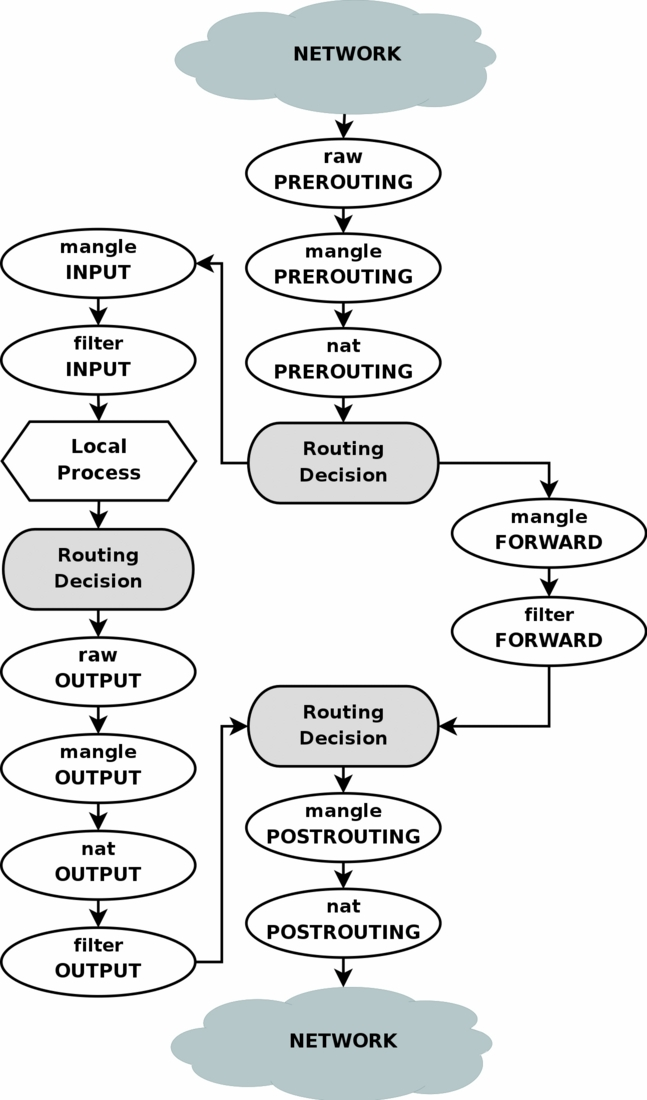
\includegraphics[width=0.7\linewidth]{ipTablesSceme}}
		\caption{Схема прохождения пакета через iptables}
		\label{fig:ipTablesScheme}
	\end{figure}
	
	\subsubsection{Основные понятия}
	
	iptables используется для проверки, модификации, перенаправления и отбрасывания пакетов. Код для фильтрации пакетов IPv4 уже встроен в ядро. Он основан на наборе \textbf{таблиц}, каждая из которых служит конкретной цели. Таблицы составляют набор предопределенных \textbf{цепочек}, которые, в свою очередь, содержат список \textbf{правил}, организованных в определенном порядке. Каждое правило состоит из критерия (набора условий) и действия, которое применяется к пакетам, подпадающим под этот критерий, то есть, если все условия выполнены. iptables является утилитой, которая позволяет работать с этими цепочками и правилами.

	\begin{itemize}
		\item \textbf{Таблица} -- совокупность базовых и пользовательских цепочек, объединенных общим функциональным назначением. Имена таблиц (как и модулей критериев) записываются в нижнем регистре, так как в принципе не могут конфликтовать с именами пользовательских цепочек. iptables содержит пять таблиц:
			\begin{enumerate}
				\item 
				\emph{raw} используется только для настройки пакетов, поэтому они освобождаются от отслеживания.
				\item 
				\emph{filter} -- это таблица по умолчанию, в которой сосредоточены все действия типичные для межсетевых экранов.
				\item 
				\emph{nat} используется для преобразования сетевых адресов (например, проброс портов).
				\item
				\emph{mangle} служит для специальных преобразований пакетов
				\item
				\emph{security} используется для контроля доступа (например, SELinux).
			\end{enumerate}	
			Для обычной настройки межсетевого экрана достаточно использовать только две из них: filter и nat. Остальные таблицы используются лишь в сложных конфигурациях затрагивающих множество маршрутизаторов и точек маршрутизации.

		\item \textbf{Цепочка} — упорядоченная последовательность правил. Таблицы состоят из цепочек, которые состоят из списка правил, расположенных в определенном порядке. Таблица по умолчанию, filter, содержит три встроенные цепочки: INPUT, OUTPUT и FORWARD, которые активируются в разных точках процесса фильтрации пакетов, как показано на диаграмме. Таблица nat включает стандартные цепочки PREROUTING, POSTROUTING, и OUTPUT. Цепочки можно разделить на \emph{пользовательские} и \emph{базовые}.
			\begin{itemize}
				\item 
				\textbf{Базовая цепочка} -- цепочка, создаваемая по умолчанию при инициализации таблицы. Каждый пакет, в зависимости от того, предназначен ли он самому хосту, сгенерирован им или является транзитным, должен пройти положенный ему набор базовых цепочек различных таблиц. Кроме того, базовая цепочка отличается от пользовательской наличием «действия по умолчанию» (default policy). Это действие применяется к тем пакетам, которые не были обработаны другими правилами этой цепочки и вызванных из нее цепочек (см. переходы). Имена базовых цепочек всегда записываются в верхнем регистре (PREROUTING, INPUT, FORWARD, OUTPUT, POSTROUTING).
				\item 
				\textbf{Пользовательская цепочка} -- цепочка, созданная пользователем. Может использоваться только в пределах своей таблицы. Рекомендуется не использовать для таких цепочек имена в верхнем регистре, чтобы избежать путаницы с базовыми цепочками и встроенными действиями. Пользовательские цепочки могут быть добавлены для упорядочивания наборов правил, а также для повышения эффективности работы iptables.
			\end{itemize}
			По умолчанию, все цепочки пустые и не содержат каких-либо правил. У цепочек, однако, есть стандартное правило (\emph{политика}), которое в основном имеет действие ACCEPT, но может (и должно) быть изменено на DROP, если нужно быть уверенным в том, что даже если пакет проскочит сквозь набор установленных правил, он будет отброшен. Стандартное правило применяется к пакетам только тогда, когда они достигают конца цепочки, пройдя по остальным правилам.
		\item 
		\textbf{Правило.} Фильтрация пакетов основана на правилах, каждое из которых задается набором \textbf{условий} и целевым \textbf{действием}. Если пакет соответствует всем условиям, к нему будет применено указанное действие. Типовые условия могут проверять, например, с какого интерфейса пришел пакет (например, eth0 или eth1), какого он типа (ICMP, TCP или UDP), или на какой порт пакет направляется. Правило состоит из \emph{критерия}, \emph{действия} и \emph{счетчика}.
			\begin{itemize}
				\item 
				\textbf{Критерий} — логическое выражение, анализирующее свойства пакета и/или соединения и определяющее, подпадает ли данный конкретный пакет под действие текущего правила.
				\item 
				\textbf{Действие} — описание действия, которое нужно проделать с пакетом и/или соединением в том случае, если они подпадают под действие этого правила. О действиях более подробно будет рассказано ниже.
				\item 
				\textbf{Счетчик} — компонент правила, обеспечивающий учет количества пакетов, которые попали под критерий данного правила. Также счетчик учитывает суммарный объем таких пакетов в байтах.
			\end{itemize}
		Если пакет соответствует критерию, к нему применяется действие, и он учитывается счетчиком. Критерия может и не быть — тогда неявно предполагается критерий «все пакеты». Указывать действие тоже не обязательно — в отсутствие действия правило будет работать только как счетчик. Целевое действие указывается с помощью опций -j или -- -jump. Действием может быть одно из стандартных действий, действий расширений или переход на пользовательскую цепочку. Стандартные действия включают ACCEPT, DROP, QUEUE и RETURN. Примерами действия расширений могут быть REJECT и LOG. Если применено одно из стандартных действий, участь пакета решается незамедлительно и обработка пакета в таблице прекращается. Если действием указан переход на пользовательскую цепочку, и пакет проходит через нее, он возвращается на исходную цепочку и продолжает со следующего после перехода правила. Действия расширений могут быть \emph{терминальными} (как стандартные действия) или \emph{нетерминальными} (как пользовательские цепочки).
		
		\item 
		\textbf{Прохождение по цепочке.} Принятый на сетевом интерфейсе пакет проходит по цепочкам таблиц в порядке, изображенном на диаграмме (Рис. \ref{fig:ipTablesScheme}). На первой точке маршрутизации (routing decision) принимается решение, направляется ли пакет на локальную машину (в таком случае пакет проходит через цепочки INPUT) или куда-то в другое место (в этом случае пакет проходит через цепочки FORWARD). На второй точке маршрутизации принимается решение, на какой сетевой интерфейс перенаправить исходящий пакет. В каждой цепочке по пути следования пакета, для каждого из правил, в которых удовлетворяются все условия, выполняется соответствующее действие. Три наиболее часто используемые действия -- ACCEPT, DROP и переход на пользовательскую цепочку. В противоположность стандартным цепочкам, которые имеют действия по умолчанию, цепочки пользователя такого действия не имеют. Если не удовлетворены условия ни одного из правил пользовательской цепочки, пакет возвращается обратно в вызвавшую ее цепочку, как изображено на Рис.\ref{fig:packageRet}. Если в какое-то время выполнились все условия цепочки с действием DROP, пакет немедленно отбрасывается и над ним более не производится никаких действий.
			\begin{figure}[h]
				\center{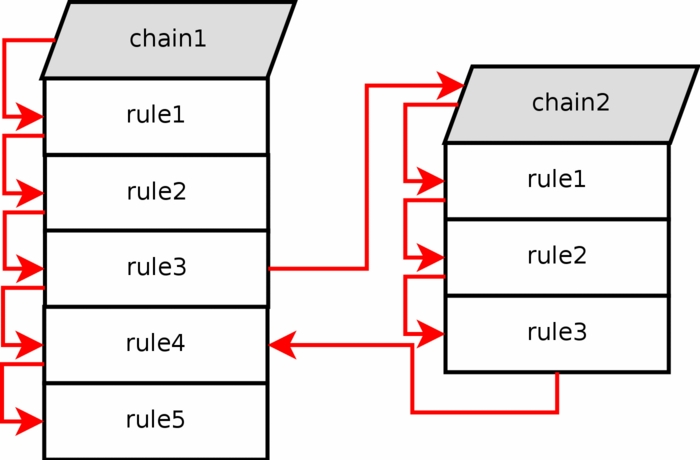
\includegraphics[width=0.7\linewidth]{packageRet}}
				\caption{Схема возвращения пакета обратно в вызвавшую ее цепочку}
				\label{fig:packageRet}
			\end{figure}
		\item 
		\textbf{Модули.} Существует множество модулей которые могут использоваться для расширения возможностей iptables, такие как \emph{connlimit}, \emph{conntrack}, \emph{limit} и \emph{recent}. Эти модули дополняют iptables новой функциональностью для того, чтобы были возможны более сложные правила фильтрации.
	\end{itemize}

	\subsubsection{Принцип работы}
	
	Все пакеты пропускаются через определенные для них последовательности цепочек (см. Рис. \ref{fig:ipTablesScheme}). При прохождении пакетом цепочки, к нему последовательно применяются все правила этой цепочки в порядке их следования. Под применением правила понимается: во-первых, проверка пакета на соответствие критерию, и во-вторых, если пакет этому критерию соответствует, применение к нему указанного действия. Под действием может подразумеваться как элементарная операция (встроенное действие, например, ACCEPT, MARK), так и переход в одну из пользовательских цепочек. В свою очередь, действия могут быть как терминальными, то есть прекращающими обработку пакета в рамках данной базовой цепочки (например, ACCEPT, REJECT), так и нетерминальными, то есть не прерывающими процесса обработки пакета (MARK, TOS). Если пакет прошел через всю базовую цепочку и к нему так и не было применено ни одного терминального действия, к нему применяется действие по умолчанию для данной цепочки (обязательно терминальное).
	
	\subsection{Структура локальной (кафедральной), факультетской и университетской сетей с указанием IP и доменных адресов.}
	
		\subsubsection{Сбор информации о сети вручную.}
		
			Задачу сбора информации можно разделить на две подзадачи: определение работоспособности узла и определение его DNS-имени.
			
			Для определения работоспособности узла можно воспользоваться программой \textbf{ping}. Ping — утилита для проверки соединений в сетях на основе TCP/IP. Утилита отправляет запросы (ICMP Echo-Request) протокола ICMP указанному узлу сети и фиксирует поступающие ответы (ICMP Echo-Reply). Время между отправкой запроса и получением ответа (RTT, от англ. Round Trip Time) позволяет определять двусторонние задержки (RTT) по маршруту и частоту потери пакетов, то есть косвенно определять загруженность на каналах передачи данных и промежуточных устройствах.
			
			Обычный эхо-запрос имеет длину 64 байта (плюс 20 байт IP-заголовка). По стандарту RFC 791 IPv4 суммарный объём пакета не может превышать 65 535 байт.
			
			Полное отсутствие ICMP-ответов может также означать, что удалённый узел (или какой-либо из промежуточных маршрутизаторов) блокирует ICMP Echo-Reply или игнорирует ICMP Echo-Request.
			
			Программа ping является одним из основных диагностических средств в сетях TCP/IP и входит в поставку всех современных сетевых операционных систем. Функциональность ping также реализована в некоторых встроенных ОС маршрутизаторов.
			
			Так как для отправки ICMP-пакетов требуется создавать raw-сокеты, для выполнения программы ping в UNIX-системах необходимы права суперпользователя. Чтобы обычные пользователи могли использовать ping, в правах доступа файла /bin/ping устанавливают SUID-бит.
			
			Команда ping имеет следующий синтаксис:
			\begin{verbatim}
ping [ -LRUbdfnqrvVaAB] [ -c количество] [ -i интервал] [ -l преднагрузка] [ -p шаблон]
[ -s размер-пакета] [ -t ttl] [ -w ограничение-на-время-работы] [ -F идентификатор-потока]
[ -I адрес] [ -M указание] [ -Q тип-обслуживания] [ -S буфер-отправки]
[ -T параметр-временной-метки] [ -W время-ожидания-ответа] [ переход ...] назначение
			\end{verbatim}
			
			Опции ping:\\
\textbf{-a} -- сопровождать работу программы звуком.\\
\textbf{-A} -- адаптировать интервал между отправками пакетов к длительности их доставки и возврата. Таким образом, если только не выполняется преднагрузка, в любой момент времени может быть не больше одного пакета, на который не получен ответ. Минимальный интервал для не администратора -- 200 мс. В сетях с низким rtt данный режим эквивалентен лавинообразному.\\
\textbf{-b} -- разрешить использование широковещательного адреса в качестве целевого.\\
\textbf{-B} -- запретить изменение исходного адреса для пакетов во время работы программы. Исходный адрес определяется в начале работы ping.\\
\textbf{-c количество} -- остановить работу после передачи заданного количества пакетов ECHO\_REQUEST. Если задано ограничение-на-время-работы, программа будет ждать указанное количество ответных пакетов ECHO\_REPLY в указанный период.\\
\textbf{-d} -- устанавливает параметр SO\_DEBUG на используемый сокет. Примечание: этот параметр не используется ядром Linux.\\
\textbf{-F идентификатор-потока} -- устанавливать идентификатор-потока в отправляемых пакетах (только для ping6). Если указан нуль, идентификатор-потока будет генерироваться случайно ядром.\\
\textbf{-f} -- лавинообразный режим. Для каждого пакета ECHO\_REQUEST выводится точка (`.'), для каждого ответного пакета ECHO\_REPLY -- забой (удаление последней точки). Это позволяет наглядно представлять число потерянных пакетов. Если интервал между отправками не задан, последние производятся с наибольшей скоростью (по мере получения ответов) или со скоростью 100 раз в секунду, в зависимости от того, в каком случае получается большая скорость. Задавать нулевой интервал между отправками может только суперпользователь.\\
\textbf{-i интервал} -- интервал в секундах между отправкой пакетов. По умолчанию между отправкой пакетов делается пауза в 1 секунду, либо, в случае лавинообразного режима, отправка производится без пауз. Задавать значения меньше 0.2 может только суперпользователь.\\
\textbf{-I адрес} -- установить адрес источника в указанный. В качестве аргумента может выступать числовой IP-адрес или имя устройства. Этот параметр обязателен при отправке запросов на локально соединённый адрес IPv6.\\
\textbf{-l преднагрузка} -- послать с максимальной скоростью указанное количество пакетов, не дожидаясь ответов, и затем перейти в обычный режим работы. Значения больше 3 может указывать только суперпользователь.\\
\textbf{-L} -- подавлять циклические петли для широковещательных пакетов. Этот ключ применяется только если в качестве целевого адреса указан широковещательный.\\
\textbf{-n} -- только цифровой вывод. Не расшифровывать имена (символьный вид) адресов.\\
\textbf{-p шаблон} -- можно указать до 16 несмысловых байтов для заполнения пакетов. Это полезно при диагностике проблем в сети. Например, -p ff заполнит все пакеты единицами символами.\\
\textbf{-Q тип-обслуживания} -- разряды байта QoS (Quality of Service -- качество обслуживания) для датаграмм ICMP. Тип-обслуживания может быть либо десятичным либо шестнадцатеричным числом. Обычно (согласно RFC 1349) это значение интерпретируется так: младший (нулевой) разряд зарезервирован (сейчас используется для управления событиями при переполнении), разряды 1-4 используются для указания собственно типа обслуживания, и разряды 5-7 для приоритета (IP-предпочтения). Возможные типы обслуживания: минимизация стоимости -- 0x02, максимизация надёжности -- 0x04, максимизация пропускной способности -- 0x08 минимизация задержек -- 0x10. Одновременно можно указывать только один из четырёх перечисленных разрядов. Возможный диапазон значения приоритета -- от приоритетного (0x20) до управляемого сетью (0xe0). Для указания высокого приоритета необходимы права суперпользователем (точнее, должно быть доступна возможность CAP\_NET\_ADMIN). Разряд 0x01 можно устанавливать только если в ядре включен ECN.
В RFC 2474 этот байт переопределён как DS (Differentiated Services -- дифференцированные службы): разряды 0-1 отведены для отдельных данных (тут будет использоваться ECN) разряды 2-7 для DSCP (Differentiated Services Codepoint -- точка кода дифференцированных служб).\\
\textbf{-q} -- выводить только начальные и итоговые данные (не выводить информацию об отдельных запросах).\\
\textbf{-R} -- записывать маршрут. Для пакетов ECHO\_REQUEST будет включен параметр RECORD\_ROUTE и на экран будет выведен буфер маршрута для возвращённых пакетов. Заметим, что в заголовок IP помещается не больше 9 таких маршрутов. Многие узлы игнорируют или не отбрасывают этот параметр.\\
\textbf{-r} -- не использовать обычные таблицы маршрутизации и передавать данные прямо на компьютер, подключенный к интерфейсу. Если компьютер не находится в сети с прямым подключением, то возвращается сообщение об ошибке. Этот параметр может использоваться вместе с -I для проверки локальной системы через интерфейс, по которому не идет маршрутизация (например после того, как интерфейс был сброшен routed(8)).\\
\textbf{-s размер-пакета} -- размер пакетов для пересылки. По умолчанию -- 56, что соответствует размеру 64 байта после добавления 8 байтов заголовка ICMP.\\
\textbf{-S буфер-отправки} -- размер буфера отправки соединения. По умолчанию буферизируется не больше одного пакета.\\
\textbf{-t ttl} -- время актуальности пакета IP (ttl -- Time to Live).\\
\textbf{-T параметр-временной-метки} -- параметры временной метки IP. Возможные значения параметра-временной-метки: tsonly (только временная метка), tsandaddr (временная метка и адреса) и tsprespec хост1 [хост2 [хост3 [хост4]]] (отмечать переходы).\\
\textbf{-M указание} -- стратегия обнаружения маршрута MTU. Возможные значения: do (запретить фрагментацию, даже локальную), want (выполнять обнаружение PMTU, фрагментировать локально если размер пакета слишком большой) и dont (не устанавливать флаг DF).\\
\textbf{-U} -- выводить полное время прохода (старое поведение). По умолчанию выводится сетевое время прохода, которое может отличаться от реального, например из-за ошибок DNS.\\
\textbf{-v} -- выводить подробную информацию.\\
\textbf{-V} -- вывести информацию о версии и закончить работу.\\
\textbf{-w ограничение-на-время-работы} -- время, по истечении которого ping завершит свою работу независимо от количества посланных и принятых пакетов. При указании этого параметра время ожидания для одного пакета игнорируется и работа может быть завершена ранее указанного срока только в случае получения информации об ошибке (т.е. уведомления о том, что ответных пакетов точно не будет).\\
\textbf{-W время-ожидания-ответа} -- время ожидания (в секундах) ответного пакета. Принимается во внимание только если не было принято ни одного ответа. В противном случае программа ожидает получения двух ответов.

Для определение DNS имени узла можно воспользоваться программой \textbf{nslookup}. В ArchLinux её можно установить, установив пакет \texttt{dnsutils}. nslookup (англ. name server lookup поиск на сервере имён) — утилита, предоставляющая пользователю интерфейс командной строки для обращения к системе DNS (проще говоря, DNS-клиент). Позволяет задавать различные типы запросов и запрашивать произвольно указываемые сервера. Её аналогом являются утилиты host и dig. Разработана в составе пакета BIND (для UNIX-систем).

			Команда имеет следующий синтаксис:\\\\
			\texttt{nslookup [-option] [name| -] [server]}\\

			\textbf{Определение маршрута.}
			
			Для определения маршрута следования пакета используем программу \textbf{tracepath}, которая заменила более старую утилиту \textbf{traceroute}. Tracepath -- это служебная компьютерная программа, предназначенная для определения маршрутов следования данных в сетях TCP/IP. Программа tracepath выполняет отправку данных указанному узлу сети, при этом отображая сведения о всех промежуточных маршрутизаторах, через которые прошли данные на пути к целевому узлу. В случае проблем при доставке данных до какого-либо узла программа позволяет определить, на каком именно участке сети возникли неполадки.
			
			Для определения промежуточных маршрутизаторов tracepath отправляет целевому узлу серию ICMP-пакетов (по умолчанию 3 пакета), с каждым шагом увеличивая значение поля TTL (\emph{<<время жизни>>}) на 1. Это поле обычно указывает максимальное количество маршрутизаторов, которое может быть пройдено пакетом. Первая серия пакетов отправляется с TTL, равным 1, и поэтому первый же маршрутизатор возвращает обратно ICMP-сообщение \emph{<<time exceeded in transit>>}, указывающее на невозможность доставки данных. Traceroute фиксирует адрес маршрутизатора, а также время между отправкой пакета и получением ответа (эти сведения выводятся на монитор компьютера). Затем traceroute повторяет отправку серии пакетов, но уже с TTL, равным 2, что заставляет первый маршрутизатор уменьшить TTL пакетов на единицу и направить их ко второму маршрутизатору. Второй маршрутизатор, получив пакеты с TTL=1, так же возвращает \emph{<<time exceeded in transit>>}.
			
			Процесс повторяется до тех пор, пока пакет не достигнет целевого узла. При получении ответа от этого узла процесс трассировки считается завершённым.
			
			Синтаксис:
			
			\texttt{tracepath [-n] [-b] [-l <len>] [-p port] <destination>}
			
			Опции:
			\texttt{-n} -- выводить не DNS-имена хостов, а их IP.
			\texttt{-b} -- выводить и DNS-имена, и IP хостов.
			\texttt{-l} -- изменить начальную длину пакета (по умолчанию -- 65536)
			\texttt{-m} -- изменить максимальное количество проходимых хостов (то есть, изменить TTL), по умолчанию значение установлено на 30.
			\texttt{-p} -- изменить использующийся порт.\\
			
			Пример использования:
			\begin{verbatim}
$ tracepath -m 10 vmk.ugatu.ac.ru
 1?: [LOCALHOST]                                         pmtu 1500
 1:  my.router                                             2.329ms 
 1:  my.router                                             1.451ms 
 2:  77.79.168.3.dynamic.ufanet.ru                         2.734ms pmtu 1480
 2:  92.50.191.57.static.ufanet.ru                         2.246ms 
 3:  no reply
 4:  cmr4-te21.ufa.ufanet.ru                               2.251ms 
 5:  ckm53-1-te41.ufa.ufanet.ru                           13.307ms 
 6:  usatu-gw.ufanet.ru                                    5.704ms 
 7:  CORE-MTS.ugatu.su                                     3.567ms 
 8:  no reply
 9:  no reply
10:  no reply
     Too many hops: pmtu 1480
     Resume: pmtu 1480 
			\end{verbatim}
			
			Утилита tracepath возвращает список маршрутизаторов, в которые эхо-запрос входит. Утилита ping с ключом -R возвращает список маршрутизаторов, из которых эхо-запрос выходит.	
			
			Например:
			\begin{verbatim}
$ ping -c 3 -R vmk.ugatu.ac.ru
PING vmk.ugatu.ac.ru (193.233.146.242) 56(124) bytes of data.
64 bytes from vmk.ugatu.ac.ru (193.233.146.242): icmp_seq=1 ttl=121 time=9.43 ms
NOP
RR: 	PC (192.168.1.37)
	77.79.168.3.dynamic.ufanet.ru (77.79.168.3)
	92.50.191.57.static.ufanet.ru (92.50.191.57)
	b0-te21.ufa.ufanet.ru (92.50.191.210)
	cmr4-1-te77.ufa.ufanet.ru (92.50.190.69)
	usatu-lgw.ufanet.ru (81.30.192.241)
	MTS-G0.ugatu.su (193.233.144.66)
	10.61.4.254
	vmk.ugatu.ac.ru (193.233.146.242)

64 bytes from vmk.ugatu.ac.ru (193.233.146.242): icmp_seq=2 ttl=121 time=14.9 ms
NOP	(same route)
64 bytes from vmk.ugatu.ac.ru (193.233.146.242): icmp_seq=3 ttl=121 time=18.7 ms
NOP	(same route)

--- vmk.ugatu.ac.ru ping statistics ---
3 packets transmitted, 3 received, 0% packet loss, time 2002ms
rtt min/avg/max/mdev = 9.431/14.362/18.740/3.820 ms

			\end{verbatim}
			
		\subsubsection{Сбор информации о сети с помощью специального приложения}

			Сбор информации о сети можно разделить на две подзадачи: ввод диапазона адресов и определение работоспособности узла и его доменного имени.\\
			
			\textbf{Ввод диапазона адресов.}
			
			Для упрощения процесса сбора информации о сети, необходимо предусмотреть возможность ввода в нескольких адресов или диапазона, путем ввода начального и конечного адреса. Современные среды разработки предоставляют большое количество компонент, позволяющих организовать ввод: например, компонент в виде пары <<текстовое поле -- пара кнопок со стрелками>> или поля для текстового ввода (\emph{LineEdit}). Для приложения по сбору и анализу информации о сети было принято решение использовать компонент, в виде <<поля для текстового ввода>>.
			
			Однако, если указывается диапазон значений, то необходимо сгенерировать все адреса от начального до конечного. Это можно сделать путем создания адресов от начального до конечного при помощи цикла.\\

			\textbf{Обобщенный алгоритм решения.}
			
			\begin{enumerate}
				\item Считать значения с компонент выбора диапазонов.
				\item Преобразовать значения с соответствующих компонент в IP-адрес.
				\item Сгенерировать диапазон адресов от начального до конечного.				
			\end{enumerate}
			
			\textbf{Определение работоспособности узла и DNS-имени узла.} Для определения работоспособности узла необходимо использовать raw-сокеты, посылающие ICMP-пакеты. Их использование требует прав суперпользователя.
			
			Рассмотрим методы решения задачи определения работоспособности узла. 
			
			Существуют языки программирования, которые предоставляет встроенные решения для определения работоспособности узла, например, пространство имён \texttt{Ping} в платформе .NET и функция\texttt{InetAddress.isReachable()} в языке Java, однако в большинстве языков встроенных решений для этой задачи нет. В таком случае можно воспльзоваться одним из двух возможных методов решения: 
			
			\begin{enumerate}
				\item Использование сиситемного пинга. Данный метод предполагает запуск программы ping, входящей в состав операционной системы. Реализация данного метода может потребовать анализа выходного потока программы или кода её завершения, с целью получения информации о работоспособности узла.
				\item Прямое формирование ICMP пакета и отправка его с помощью raw-сокетов. Данный метод достаточно сложен, так как его использование предполагает высокие познания в ICMP-пакетах, однако можно воспользоваться готовой реализацией из одного из open-source пректов.	
			\end{enumerate}
			 
			
			%%%%%%%%%%%%%%%%%%%%%%%%%%%%%%%%%%%%%%%%%%%
			
			Расмотрим способы определения DNS-имени узла.
			
			\begin{itemize}
			
				\item \textbf{В операционнлй сисистеме Windows} необходимо открыть сокет и обратиться к функции WinApi
				\begin{lstlisting}					
int WSAAPI getnameinfo(
  _In_  const struct sockaddr FAR *sa,
  _In_  socklen_t                 salen,
  _Out_ char FAR                  *host,
  _In_  DWORD                     hostlen,
  _Out_ char FAR                  *serv,
  _In_  DWORD                     servlen,
  _In_  int                       flags
);
				\end{lstlisting}
				
				в которой \texttt{sa} -- указатель на открытый сокет, \texttt{salen} -- длина структуры, на которую указывает \texttt{sa}, host -- указатель, по которому запишется информация о найденом DNS-имени, \texttt{hostlen} -- длина выделенного под имя буфера, \texttt{serv} -- указатель, в который будет записана информация об имени сервиса, \texttt{servlen}, длина выделенного под имя сервиса буфера, \texttt{flags} -- флаги этой функции.
				
				\item \textbf{В операционной системе семейства GNU/Linux} необходимо использовать функцию 
				
				\begin{lstlisting}					
struct hostent *gethostbyaddr(const void *addr,
                              socklen_t len, 
                              int type);
				\end{lstlisting}
				
				которая возвращает структуру типа \texttt{hostent} указанному адресу машины \texttt{addr}, длина которого равна \texttt{len}, а тип адреса равен \texttt{type}.
			%	\item{\textbf{Системный ping}}. Данный метод предполагает запуск программы ping, входящей в состав операционной системы. Реализация данного метода может потребовать анализа выходного потока программы, с целью получения информации о работоспособности узла (или его неработоспособности). Другая реализация данноо метода может потребовать анализа не текста, а кода завершения программы. Недостаток такого метода -- усложнение программы для работы на различных операционных системах из-за отличий в синтаксисе.
			%	\item{\textbf{Использование raw-сокетов}}. Данный метод предполагает написание библиотеки (модуля или утилиты), который формирует ICMP пакет и отправляет его через RAW-сокет. Недостатком можно считать сложность реализации библиотеки такого типа, а также необходимость в правах суперпользователя.
			%	\item{\textbf{Использование библиотек выбранного языка}}. Данный метод является наиболее простым в реализации, так как он подразумевает использование уже готовых библиотек для определения работоспособности узла. Однако, так как библиотеки также реализуют интерфейс для работы с raw-сокетами, этот метод тоже требует прав суперпользователя.
			%	Примеры таких библиотек:
				
			%	\begin{enumerate}
			%	\item Написанная на ANCI-C библиотека libping.
			%	\item Написанный на PHP класс
			%	\end{enumerate}
			\end{itemize}
			
			Для этих функций существуют различные кроссплатформенные и не кроссплатформенные обертки, например, \texttt{socket.gethostbyaddr()} в стандартной библиотеке языка Python, \texttt{gethostbyaddr} в PHP, \texttt{QHostInfo ::hostName()} во фреймворке Qt, \texttt{System.Net.Dns.GetHostByAddress()} в платформе .NET и другие.
			
			%%ЗДЕСЬ
			
			Для удобной работы с приложением, а также для повышения скорости его работы необходимо предусмотреть следующее: при большом диапазоне адресов для обработки всего количества потребуется довольно много времени. При этом, в обычном случае, блокируется основной поток программы, программа <<зависает>>. Кроме того, большую часть времени программа проводит в ожидании ответа и не совершает работы. Для решения данных проблем существует два подхода: использование ассинхронных вызовов и многопоточность.
			
			\begin{itemize}
				\item {\textbf{Многопоточная модель}}. При многопоточном подходе приложение создает некоторое количество потоков (пул), передавая каждому из них задачу и данные для обработки. Задачи выполняются параллельно. Если потоки не имеют общих данных, то у нас не будет накладных расходов на синхронизацию, что делает работу достаточно быстрой. После завершения работы поток не убивается, а лежит в пуле, ожидая следующей задачи. Это убирает накладные расходы на создание и удаление потоков. Потоков может быть достаточно большое количество, медленные запросы забирают поток надолго, быстрые -- обрабатываются почти мгновенно, освобождая поток для другой работы. Это не позволяет медленным запросам забирать все процессорное время, заставляя подвисать быстрые запросы. Но у такой системы есть определенные ограничения. Может возникнуть ситуация, когда останется большое количество медленных запросов, например работающих с БД или файловой системой. Такие запросы заберут себе все потоки, что сделает невозможным выполнение других запросов. Даже если запросу нужно всего 1мс на выполнение -- он не будет вовремя обработан. Это можно решить увеличением числа потоков, чтобы они могли обработать достаточно большое количество медленных запросов. Однако, чем больше потоков мы создаем, тем больше накладных расходов на их обработку и тем меньше процессорного времени выделяется каждому потоку.
				\item {\textbf{Асинхронная модель}}. Менее распространенная модель, нежели многопоточная, но имеющая не меньшие возможности. Асинхронная модель построена на очереди событий (\emph{event-loop}). При возникновении некоторого события (пришел запрос, выполнилось считывание файла, пришел ответ от БД) оно помещается в конец очереди. Поток, который обрабатывает эту очередь, берет событие с начала очереди и выполняет связанный с этим событием код. Пока очередь не пуста процессор будет занят работой. И имеется единственный поток, обрабатывающий очередь событий. Почти все операции неблокирующие. Блокирующие тоже имеются, но их использование крайне не рекомендуется. Асинхронное приложение с неблокирующими операциями использует процессорное время гораздо эффективнее, но более сложно при проектировании. Особенно сильно это сказывается на утечках памяти.
			%	\item{\textbf{Асинхронный вызов}}. Асинхронный метод -- это метод, который не задерживает выполнение программы пока он ждёт результатов выполнения какой-либо функции.
			%	\item{\textbf{Многопоточность}}. Многопоточность -- это свойство платформы (например, операционной системы, виртуальной машины и т. д.) или приложения, состоящее в том, что процесс, порождённый в операционной системе, может состоять из нескольких потоков, выполняющихся <<параллельно>>, то есть без предписанного порядка во времени. При выполнении некоторых задач такое разделение может достичь более эффективного использования ресурсов вычислительной машины. Сутью многопоточности является квазимногозадачность на уровне одного исполняемого процесса, то есть все потоки выполняются в адресном пространстве процесса. Кроме этого, все потоки процесса имеют не только общее адресное пространство, но и общие дескрипторы файлов. Выполняющийся процесс имеет как минимум один (главный) поток. В программе в главном потоке находится графический интерфейс, а вызов функций выполняется в отдельных потоках, тем самым не блокируя главный поток.
			\end{itemize}
			В различных языках программирования присутствуют различные библиотеки, позволяющие использовать асинхронность и многопоточность.
			
			\begin{itemize}
				\item  \textbf{Node.js} -- программная платформа для языка JavaScript. В основе Node.js лежит событийно-ориентированное и асинхронное программирование с неблокирующим вводом/выводом.
				\item В языке \textbf{Java} поток представляется в виде объекта-потомка класса \texttt{Thread}. Этот класс инкапсулирует стандартные механизмы работы с потоком. Также в Java присутствует асинхронность в виде класса \texttt{AsyncTask}.
				\item В языке \textbf{Python} многопоточность реализована в модулях \texttt{Thread}. Однако, при работе с потоками необходимо учитывать такое явление, как GIL -- глобальная блокировка интерпретатора. Также можно использовать модуль {multiprocessing}, котры позволяет запускать подпрограммы как отдельные процессы ОС. С версии 3.5, вышедшей 13 сентября 2015 года, сопрограмма в Python является специальным объектом native coroutine, что позволило добавить возможность асинхронных вызовов, для этого используется ключевые слова \texttt{async} и \texttt{await}.
				\item В языке \textbf{C++11} многопоточность представлена в пространстве имен \texttt{std::thread} в библиотеке thread. Именно там содержатся классы реализующие многопоточность, в частности класс \texttt{thread}.
				\item В фреймворке \textbf{Qt} многопоточность представленна классом \texttt{Thread}, однако его использование сильно усложнено необходимостью запускать новый поток с помощью системы \texttt{signal/slot}.
				\item В платформе \textbf{.NET} многопоточность представлена в пространстве имен \texttt{System.Threading}. Именно там содержатся классы реализующие многопоточность, в частности класс \texttt{Thread}. Асинхронное программирование реализовано с помощью \texttt{async/await}.		
				\item Модель многопоточности языка \textbf{Go} была создана на основе CSP\emph{(англ. Communicating sequential processes)} Тони Хоара, но также присутствуют такие особенности Пи-исчисления, как канальная передача. Go дает возможность создать новый поток выполнения программы (go-процедуру) с помощью ключевого слова \texttt{go}, которое запускает анонимную или именованную функцию в заново созданной go-процедуре (аналог \textbf{coroutine}). Все go-процедуры в рамках одного процесса используют общее адресное пространство, выполняясь над ОС-потоками, но без жёсткой привязки к последним, что позволяет выполняющейся go-процедуре покидать поток с заблокированной go-процедурой (ждущей, например, отправки или приема сообщения из канала) и продолжать работу далее.
				\item В языке \textbf{Erlang} используются облегчёные процессоы в соответствии с моделью акторов. Такой подход позволяет выполнять одновременно сотни тысяч и даже миллионы таких процессов, каждый из которых может иметь скромные требования по памяти. Процессы изолированы друг от друга и не имеют общего состояния, но между ними можно установить связь и получать сообщения об их состоянии. Для взаимодействия процессов используется асинхронный обмен сообщениями. Каждый процесс имеет свою очередь сообщений, обработка которой использует сопоставление с образцом.
				\begin{figure}[H]
					\center{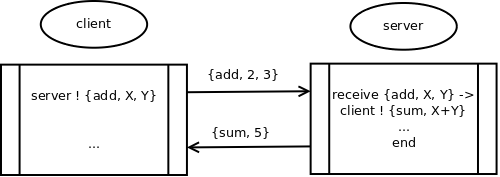
\includegraphics[width=0.7\linewidth]{ErlangThread}}
					\caption{Обмен сообщениями между процессами в Erlang.}
				\label{fig:ErlangThread}
			\end{figure}
		\end{itemize}
		
		Для решения поставленных задач по определению работоспособности узла и определнию его доменного имени было принято решение использовать стандартные библиотеки языка; в качестве метода распараллеливания был выбран многопоточный подход.
		
		Таким образом, обобщенный алгоритм решения можно представить следующим образом:
		
		\begin{enumerate}
			\item 
			Создать поток для обработки каждого адреса из диапазона.
			\item 
			В каждом потоке:
			\begin{enumerate}
				\item Определить работоспособность узла
				\item Определить DNS-имя узла
			\end{enumerate}
		\end{enumerate}
		
		\subsubsection{Анализ информации о сети}
		
		Под анализом сети понимается определение маски подсети, адреса сети и широковещательного адреса.
		
		\begin{enumerate}
			\item
				\textbf{Получение маски}. В терминологии сетей TCP/IP маской подсети или маской сети называется битовая маска, определяющая, какая часть IP-адреса узла сети относится к адресу сети, а какая — к адресу самого узла в этой сети. Для начала необходимо определить минимальный размер сети. У всех адресов некоторой подсети будет одинаковая часть, относящаяся к адресу сети, оставишеся биты относятся к адресу узла. Зная количество бит, относящихся к адресу узла, можно определить минимальный размер сети. Одинаковая часть, которая относится к адресу сети, будет одинакова. Следовательно, в маске сети соответствующая часть, описывающая адрес сети, будет состоять из 1, а оставшаяся часть, отвечающая за адрес узла, из 0.

			Для получения маски, следует побитово, слева на право, сравнивать в двоичной системе начальный и конечный адреса из диапазона. Если биты совпадают, пишем в маску 1. Как только найдено первое несовпадение, пишем в маску 0 и оставшуюся маску заполняем нулями. Например:

			\begin{tabular}{|c|cccc|}
			\hline
				Начальный адрес(192.233.146.242): & 11000001 & 11101001 & 10010010 & 11110010\\
				Конечный адрес (192.233.146.245): & 11000001 & 11101001&10010010 & 11110101\\
			\hline
				Маска подсети (255.255.255.248): & 11111111&11111111 & 11111111 & 11111000\\
			\hline
			\end{tabular}

			\item
				\textbf{Определение адреса сети}. Адрес сети -- самый младший адрес в сети. Он используетсся, когда требуется  указать  всю сеть целиком, например, когда задается маршрутизация до этой сети. Адрес сети -- первый адрес в сети. Так как адрес сети тоже принадлежит сети, то его сетевая часть совпадает с сетевой частью других адресов диапазона, однако его машинная часть состоит полностью из 0. Соответственно, чтобы определить адрес сети, нам достаточно обнулить машинную часть любого адреса из диапазона.

				Адрес сети можно определить произведя поразрядную конъюнкцию маски сети и адресом любого хоста-компьютера. Это приведет к обнулению машинной части адреса и получению его сетевого адреса. Например:

		
				\begin{tabular}{|c|cccc|}
				\hline
					Адрес узла (192.233.146.245): & 11000001 & 11101001 & 10010010 & 11110101\\
					Маска подсети (255.255.255.248): & 11111111 & 11111111 & 11111111 & 11111000\\
				\hline
					Адрес сети (193.233.146.240): & 11000001 & 11101001 & 10010010 & 11110000\\
				\hline
				\end{tabular}
				\item
					\textbf{Определение широковещательного адреса}. Широковещательный адрес позволяет системе посылать сообщение одновременно всем системам в сети. Это всегда последний адрес в сети. Другими словами, это адрес, у которого машинная часть состоит полностью из 1.

				Широковещательный адрес можно определить путем поразрядной дизъюнкции любого адреса из сети и инвертированной маски сети. Инвертировав маску сети мы получим в сетевой части нули, а в машинной -- единицы. Проведя побитовое сложение инвертированной маски с любым адресом из диапазона получим, что сетевая часть останется неизменной, а машинная заполнится единицами. Например:

			\begin{tabular}{|c|cccc|}
			\hline
				Маска подсети (255.255.255.248): & 11111111 & 11111111 & 11111111 & 11111000\\
			Инверсия маски (0.0.0.3): & 00000000 & 00000000 & 00000000 & 00000111\\
				Адрес узла (192.233.146.245): & 11000001 & 11101001 & 10010010 & 11110101\\
			\hline
				Широковещательный адрес (193.233.146.247): & 11000001 & 11101001 & 10010010 & 11110111\\
			\hline
			\end{tabular}


			\item
				\textbf{Адрес шлюза}. Обычно адрес шлюза -- первый адрес сети, следует сразу за адресом сети. Для его нахождения достаточно прибавить к адресу сети единицу.

				\begin{tabular}{|c|cccc|}
				\hline
					Адрес сети (193.233.146.240): & 11000001 & 11101001 & 10010010 & 11110000\\
				\hline
					Адрес шлюза (192.233.146.241): & 11000001 & 11101001 & 10010010 & 11110001\\
				\hline
				\end{tabular}
		\end{enumerate}
		
		\textbf{Обобщенный алгоритм решения}:
		
		\begin{enumerate}
			\item
				\textbf{Нахождение маски подсети}
				\begin{enumerate}
					\item Представить начальный и конечный адрес диапазона в двоичном виде.
					\item Произвести поразрядное сравнение начального и конечного адресов. Если значение разрядов совпадают, то соответствующий разряд маски равен 1. Иначе прерываем сравнение и в оставшиеся разряды устанавливаем 0.
				\end{enumerate}
			\item
				\textbf{Нахождение адреса сети}
				\begin{enumerate}
					\itemПредставить маску подсети и один из адресов диапазона в двоичном виде.
					\itemПроизвести поразрядную конъюнкцию маски подсети и одного из адресов диапазона.
				\end{enumerate}

			\item
				\textbf{Нахождение широковещательного адреса}
				\begin{enumerate}
					\itemПредставить маску подсети и адрес сети в двоичном виде.
					\itemПроизвести инверсию маски подсети.
					\itemПроизвести поразрядную дизъюнкцию инвертированной маски подсети и адреса сети.
				\end{enumerate}

			\item
				\textbf{Нахождение адреса шлюза}
				\begin{enumerate}
					\item Представить адрес сети в двоичном виде.
					\item Прибавить к адресу сети единицу.
				\end{enumerate}
		\end{enumerate}
		
		\subsubsection{Построение карты сети}
		
		Основой сети университета является оптоволоконное кольцо. К нему подсоединены сетевые коммутаторы, обеспечивающие переход на витую пару. К коммутаторам подсоединены кафедральные сервера, которые, в свою очередь, могут являться маршрутизаторами. К серверам через хабы или напрямую подключены остальные компьютеры.
		
	\section{Описание и реализация применяемых методов}
		\subsection{Параметры настройки TCP/IP в системе ArchLinux}
		
		Настроим статический IP-адрес для интерфейса wlo1. Зададим IP-адрес равный \texttt{192.168.1.2} с маской в 24 бита и широковещательный адрес равный \texttt{192.168.1.255}, используя утилиту ip: 
		
		\texttt{\# ip addr add 192.168.1.2/24 broadcast 192.168.1.255 dev wlo1}\\
				
		Результат выполнения команды:
		\begin{verbatim}
$ ip addr
wlo1: <BROADCAST,MULTICAST,UP,LOWER_UP> mtu 1500 qdisc mq state UP group default qlen 1000
    link/ether bc:85:56:98:73:29 brd ff:ff:ff:ff:ff:ff
    inet 192.168.1.2/24 brd 192.168.1.255 scope global wlo1
       valid_lft forever preferred_lft forever
    inet6 fe80::be85:56ff:fe98:7329/64 scope link 
       valid_lft forever preferred_lft forever
		\end{verbatim}
		
		Не будем специально задавать адрес шлюза, оставим \textbf{шлюз по умолчанию}.
		
		С помощью утилиты \texttt{drill} настроим DNS (используем, например, DNS от Google, 8.8.8.8):\\
		
		\texttt{\$ drill 8.8.8.8}
		
		Результат работы (/etc/resolv.conf):
		\begin{verbatim}
nameserver 192.168.1.1
		\end{verbatim}
		

		\subsection{Параметры настройки межсетевого экрана в системе ArchLinux}
		
		Создадим необходимые правила для межсетевого экрана с помощью iptables. Для того, чтобы посмотреть текущий набор правил и количество срабатываний каждого, можно использовать команду \texttt{iptables -nvL}:
		\begin{verbatim}
# iptables -nvL
	Chain INPUT (policy ACCEPT 1 packets, 1450 bytes)
	 pkts bytes target     prot opt in     out     source               	destination         

	Chain FORWARD (policy ACCEPT 0 packets, 0 bytes)
	 pkts bytes target     prot opt in     out     source               	destination         

Chain OUTPUT (policy ACCEPT 0 packets, 0 bytes)
 pkts bytes target     prot opt in     out     source               destination     

		\end{verbatim}
		 
		
		\subsubsection{Сброс текущих настроек}
		
		Сбросим текущие настройки, используя команды:	
		\begin{verbatim}
# iptables -F
# iptables -X
# iptables -t nat -F
# iptables -t nat -X
# iptables -t mangle -F
# iptables -t mangle -X
# iptables -t raw -F
# iptables -t raw -X
# iptables -t security -F
# iptables -t security -X
# iptables -P INPUT ACCEPT
# iptables -P FORWARD ACCEPT
# iptables -P OUTPUT ACCEPT
		\end{verbatim}
		
		\subsubsection{Редактирование правил}
		
		\textbf{Общие настройки.}
		
		\begin{enumerate}
		
			\item Цепочка \textbf{INPUT}.
			
				Первое правило будет принимать все ICMP сообщения. Некоторые ICMP сообщения очень важны, некоторые менее важны (как эхо-запросы (Pings), но никто из за них не пострадал, так что в целом это хорошая идея -- не блокировать их:
				\begin{verbatim}
# iptables -A INPUT -p icmp -j ACCEPT
				\end{verbatim}	
				Следующее правило позволит убедится в том, что никакая часть трафика, принадлежащего к уже установленным соединениям не будет отброшена (dropped).	
				\begin{verbatim}
# iptables -A INPUT -m state --state RELATED,ESTABLISHED -j ACCEPT
				\end{verbatim}
				В большинстве случаев, мы не хотим отбрасывать все входящие соединения, и именно поэтому мы настраиваем две выборочные цепочки open и interfaces. Поэтому мы добавим правило для каждой из них:
				\begin{verbatim}
# iptables -A INPUT -j interfaces
# iptables -A INPUT -j open
				\end{verbatim}		
				Теперь, последними двумя правилами, отбрасываем все, что не было явно разрешено выше. Для TCP пакетов, запрещаем подключения с tcp-reset. Входящим UDP пакетам отвечают ICMP сообщениями.	
				\begin{verbatim}
# iptables -A INPUT -p tcp -j REJECT --reject-with tcp-reset 
# iptables -A INPUT -p udp -j REJECT --reject-with icmp-port-unreachable 
				\end{verbatim}		
				Все другие протоколы, кроме TCP, UDP and ICMP будут отброшены (если они не соответствовали правилам выше). Мы делаем это путем установки к цепочке INPUT политики DROP:
				\begin{verbatim}
# iptables -P INPUT DROP		
				\end{verbatim}			
		
			\item Цепочка \textbf{FORWARD}.
			
				Просто устанавливаем к цепочке FORWARD политику DROP:		
				\begin{verbatim}
# iptables -P FORWARD DROP	
				\end{verbatim}	
				
			\item Цепочка \textbf{OUTPUT}.
			
				В общем случае не требуется фильтровать весь исходящий трафик, поскольку это сделало бы настройку намного более сложной и потребовало бы дополнительных вычислительных мощностей. Поэтому устанавливаем к цепочке OUTPUT политику ACCEPT.
				\begin{verbatim}
# iptables -P OUTPUT ACCEPT
				\end{verbatim}
				
			\item Цепочка \textbf{interfaces}.
			
				Мы будем использовать цепочку interfaces для всего трафика из надежных сетевых интерфейсов. Первое необходимое правило:		
				\begin{verbatim}
# iptables -A interfaces -i lo -j ACCEPT
				\end{verbatim}	
				
			\item Цепочка \textbf{Open}.
			
				Если необходимо принимать SSH-соединения на любых сетевых интерфейсах, нужно добавить это правило:	
				\begin{verbatim}
# iptables -A interfaces -i lo -j ACCEPT
				\end{verbatim}
				Однако, это не очень хорошая идея, т.к. таким образом открывается всему миру доступ к машине через 22 порт. Поэтому, ограничим то, какие машины могут подключаться по 22 порту, изменяя файл \texttt{/etc/hosts.allow}:	
				\begin{verbatim}
# Позволяем локальным пользователям подключаться через ssh
sshd: 127.0.0.1

# Разрешить эти адреса для соединения через SSH
sshd: 192.168.0.1
sshd: 172.272.0.32
				\end{verbatim}
				Разрешаем HTTP соединения через сетевой интерфейс wlo1:
				\begin{verbatim}
# iptables -A open -i wlo1 -p tcp --dport 80 -j ACCEPT
				\end{verbatim}
				
	\end{enumerate}
	
		\textbf{Защита от основных атак}\\
		Проверим, что новое входящее соединение является TCP SYN пакетом. В противном случае, отбросим все его пакеты:
		\begin{verbatim}
# iptables -A INPUT -p tcp ! --syn -m state --state NEW -j DROP
		\end{verbatim}
		Проверим, что пакеты не имеют входящих фрагментов. В противном случае, отбросим их:
		\begin{verbatim}
# iptables -A INPUT -f -j DROP
		\end{verbatim}
		Отбросим плохо сформироваанные XAMS-пакеты:
		\begin{verbatim}
# iptables -A INPUT -p tcp --tcp-flags ALL ALL -j DROP
		\end{verbatim}
		Удалим все NULL-пакеты:
		\begin{verbatim}
# iptables -A INPUT -p tcp --tcp-flags ALL NONE -j DROP
		\end{verbatim}
		Защитимся от <<атаки с подменой>> \emph{(англ. Spoofing attack)}:
		\begin{verbatim}
# iptables -I INPUT -i eth0 -s 10.0.0.0/8 -j DROP
# iptables -I INPUT -i eth0 -s 172.16.0.0/12 -j DROP
# iptables -I INPUT -i eth0 -s 192.168.0.0/16 -j DROP
# iptables -I INPUT -i eth0 -s 127.0.0.0/8 -j DROP
		\end{verbatim}
		
		\textbf{Создание специального правила для работы с Dropbox.}
		
		Dropbox это приложение, позволяющее хранить свои данные на серверах в облаке и делиться ими с другими устройствами через локальные сети и Интернет. Работа построена на синхронизации данных.
		
		Для синхронизации по локальной сети Dropbox использует отсылку широковещательных пакетов каждые 30 секунд всем доступным компьютерам сети. Пусть нам посчастливилось быть в одной сети с клиентами Dropbox при том, что мы сами не используем эту возможность. Создадим правило для отбрасывания таких пакетов:
		\begin{verbatim}
# iptables -A INPUT -p tcp --dport 17500 -j REJECT --reject-with icmp-port-unreachable
		\end{verbatim}

		Здесь мы использовали действие \texttt{REJECT}, а не \texttt{DROP}, так как стандарт от октября 1989 года, RFC 1122 (раздел 3.3.8), требует, чтобы хосты возвращали ошибки ICMP всегда, когда это возможно вместо простого игнорирования отбрасываемых пакетов.
		
		Теперь, скажем, мы поменяли наш взгляд касательно Dropbox и решили установить его на наш компьютер. Мы также хотим использовать возможность синхронизации по локальной сети, но только с единственным компьютером в сети, IP-адрес которого нам известен, пусть это будет, например, \texttt{10.0.0.85}. Используем ключ -R для того, чтобы заменить старое правило новым:
		\begin{verbatim}
# iptables -R INPUT 1 -p tcp --dport 17500 ! -s 10.0.0.85 -j REJECT --reject-with icmp-port-unreachable
		\end{verbatim}
		
		Теперь новое правило позволит хосту \texttt{10.0.0.85} отправить данные на порт \texttt{17500} нашего компьютера. Но теперь мы поняли, что наше правило не самое удачное: новые правила в этой цепочке смогут все равно заблокировать пакет. Мы не просто хотим пропустить пакет дальше по цепочке, а хотим сразу пометить его как принятый и пропустить в другие цепочки.
		
		Здесь мы используем ключ -I для того, чтобы вставить новое правило в самое начало цепочки, перед старым:
		\begin{verbatim}
# iptables -I INPUT -p tcp --dport 17500 -s 10.0.0.85 -j ACCEPT -m comment --comment "Friendly Dropbox:)"
		\end{verbatim}
		
		Второе правило теперь можно переписать так, чтобы оно отбрасывало пакеты, приходящие на порт \texttt{17500} с других хостов:	
		\begin{verbatim}
# iptables -R INPUT 2 -p tcp --dport 17500 -j REJECT --reject-with icmp-port-unreachable
		\end{verbatim}
		
		\subsubsection{Файл настроек}
		
		По умолчанию в Arch Linux файл с правилами iptables располагается в \texttt{/etc/iptables/iptables.rules}. Эти правила, однако, не будут загружаться автоматически при старте системы, если не включить службу \texttt{iptables.service}, которая загружает из него все правила:
		\begin{verbatim}
# systemctl enable iptables
# systemctl start iptables
		\end{verbatim}
		Когда правила добавляются через командную строку, они сохраняются лишь в оперативной памяти, и будут сброшены при перезагрузке. Чтобы выгрузить их в файл, необходимо выполнить:	
		\begin{verbatim}
# iptables-save > /etc/iptables/iptables.rules
		\end{verbatim}
		
		\subsubsection{Логирование}
		
		Действие \texttt{LOG} полезно для логирования пакетов, когда к нему применяется правило. В отличие от других действий вроде \texttt{ACCEPT} или \texttt{DROP}, \texttt{LOG} ничего не делает с пакетом, он просто продолжает свое продвижение по цепочке. Обычно условия для правила с действием \texttt{LOG} полностью дублируют условия какого-нибудь другого правила, которое следует логировать, а само логирующее правило идет непосредственно перед ним. Это значит, что, например, если нужно включить логирование всех отброшенных пакетов, следует добавить правило с действием \texttt{LOG} перед каждым правилом с \texttt{DROP}. Это не слишком удобно и плохо влияет на эффективность, поэтому можно вместо этого создать пользовательскую цепочку, например, \texttt{logdrop}:
		\begin{verbatim}
# iptables -N logdrop
		\end{verbatim}
		И добавить в нее следующие правила:
		\begin{verbatim}
# iptables -A logdrop -m limit --limit 5/m --limit-burst 10 -j LOG
# iptables -A logdrop -j DROP
		\end{verbatim}
		Теперь, когда мы захотим отбросить пакет и добавить запись в лог об этом, мы просто выполним переход на цепочку \texttt{logdrop}:
		\begin{verbatim}
# iptables -A INPUT -m conntrack --ctstate INVALID -j logdrop
		\end{verbatim}
		% IP адрес, маска сети, шлюз, параметры DNS)
		
		\subsubsection{Просмотр логированных пакетов}
		
		Логированные пакеты сохраняются как сообщения ядра в журнале systemd.
		
		Отобразить все пакеты, которые были залогированы с момента последнего перезапуска, можно выполнив команду:
		
		\begin{verbatim}
# journalctl -k | grep "IN=.*OUT=.*" | less
		\end{verbatim}	
		
	\subsection{Структура локальной (кафедральной), факультетской и университетской сетей с указанием IP и доменных адресов}
	
	\subsubsection{Сбор информации о сети с помощью специально написанного приложения}
	
		Для хранения информации об адресе используется структура \texttt{address} с полями \texttt{ip}, \texttt{is\_up} и \texttt{name}, которые хранят информацию об ip адресе, информацию о доступности сервера и его DNS-имени соответственно. Сгенерированные адреса хранятся в списке \texttt{addresses}.
			
		\textbf{Ввод и генерация диапазона адресов.}
		
		Ввод границ рассматриваемого диапазона осуществляется через компонент ввода LineEdit (текстовое поле с заданной маской ввода вида "000.000.000.000;"). Метод \texttt{text()} возвращает текущее значение в виде строки. 
	
		\textbf{Укрупненный алгоритм ввода диапазона адресов.}

\begin{verbatim}
1. Считать начальный адрес диапазона с компонент выбора.
2. Считать конечный адрес диапазона с компонент выбора.
3. Сгенерировать диапазон значений от начального до конечного адреса.
\end{verbatim}

		\textbf{Детализированный алгоритм ввода диапазона адресов.}

		\begin{enumerate}
			 \item 
			 	С первого компонента LineEdit считать начальный адрес:
			 	\begin{verbatim}
begin = lineEdit.text()
				\end{verbatim}	
			 \item 
			 	Со второго компонента LineEdit считать конечный адрес.
			 	\begin{verbatim}
end = lineEdit.text()
				\end{verbatim}		
			\item
				До тех пор, пока начальный адрес не станет равным конечному, будем заносить адрес begin в список и увеличивать адрес begin:
				\begin{verbatim}
while begin <= end:
     addresses.append(begin)
     begin = begin + 1
				\end{verbatim} 	 	
		\end{enumerate}
		
		\textbf{Сбор информации о сети.}
		
			\begin{longtable}{|p{6cm}|p{10cm}|}
			\hline
				\multicolumn{2}{|p{15cm}|}{Модуль \texttt{multiprocessing} предоставляет высокоуровневый для работы с системными потоками. Включает в себя класс \texttt{Process}.}\\
			\hline
				\texttt{Process(group=None, target=None, name=None, args=(), kwargs={}, *, daemon=None)} & Конструктор класса Process. Создает новый поток, в котором начнет выполнение функции target, аргументами которой являются объекты args.\\
			\hline
				\texttt{Process.start()} & Запуск нового потока.\\
			\hline
				\multicolumn{2}{|p{15cm}|}{Модуль \texttt{pinging} реализует системный пинг.}\\
			\hline
				\texttt{pinging.is\_up(ip, timeout)} & Осуществляет проверку работоспособности хоста. Аргументы: ip -- ip-адрес проверяемого узла, timeout -- период ожидания ответа. Возвращает True в случае успеха и False в обратном случае.\\
			\hline
				\multicolumn{2}{|p{15cm}|}{Модуль \texttt{socket} предоставляет интерфейс для работы с сокетами. Предоставляет функции для работы с сетевыми соединениями.}\\
			\hline
				\texttt{socket.gethostbyaddr(addres)} & Возвращает DNS-имя аргумента -- ip-адреса.\\
			\hline
			\caption{Функции для сбора информации о сети}
		\end{longtable}
		
		\textbf{Детализированный алгоритм сбора информации о сети.}
	\begin{verbatim}
1. Для каждого address из addresses:
2.     p = Process(ping.is_up, address.ip)
3.     p.start()
4.     Если результат ping.is_up равен True:
5.         Узел работоспособен, address.is_up = true
6.     Иначе:
7.         Узел неработоспособен, address.is_up = false
8.     address.name = socket.gethostbyaddr(адрес)
\end{verbatim}

	\textbf{Анализ сети.}

\begin{center}
\begin{longtable}{|p{6cm}|p{10cm}|}
\hline
\multicolumn{2}{|p{15cm}|}{Модуль \texttt{struct} предоставляет функции для преобразования строк в упакованные двоичные данные.}\\
\hline
\texttt{int struct.unpack(string format,bytearray arg)}&Возвращает кортеж. На первой позиции находится строка, включающая в себя значение bytearray , распакованное согласно значению аргумента format. format -- строка, состоящая из символов, первый из которых определяет порядок следования байтов, а второй тип данных, соответствующий аргументам v1,v2... В частности, format = '>I' означает, что порядок следования байт big-endian (символ '>') и данные типа unsigned int (символ "I").\\
\hline
\texttt{string struct.pack(string format,string arg)}&Возвращает строку, равную аргументу arg, упакованному согласно первому аргументу format (в случае работы с сетевыми адреса этот аргумент равен '>I').\\
\hline
\multicolumn{2}{|p{15cm}|}{Модуль \texttt{socket} предоставляет интерфейс для работы с сокетами. Предоставляет функции для работы с сетевыми соединениями.}\\
\hline
\texttt{string socket.inet\_ntoa(string byteip)}&Преобразут 32-битный IPv4 адрес, представленный в виде строки в стандартное представление (например "192.168.0.248"). Возвращает строку.\\
\hline
\texttt{string socket.inet\_aton(string ip)}&Преобразует аргумент-строку IPv4 адреса в стандартном представлении в 32-битный упакованный двоичный формат, представленный в виде строки.\\
\hline
\texttt{string bin(var)}&Возвращает строку -- бинарное представление аргумента.\\
\hline
\texttt{string os.path.commonprefix ([string arg])}&Возвращает строку -- наибольший общий префикс аргументов.\\
\hline
\texttt{int.to\_bytes(int value,int length,string byteorder)}&Возвращает строку байтов, представляющих число. byteorder -- порядок следования байтов, length -- количество байт, value -- число для преобразования.\\
\hline
\texttt{int int(int num,int degree)}&Преобразовывает num из числа в степени счисления degree в число типа int.\\
\hline
\caption{Функции для анализа сети}
\end{longtable}
\end{center}

\textbf{Укрупненный алгоритм анализа сети.}

\begin{verbatim}
Для диапазона адресов:
    1. Определение маски:
        1.1 Устанавливаем все биты маски в 0.
        1.2 Определеяем наибольший общий префикс первого и последнего адреса диапазона.
        1.3 Устанавливаем в 1 количество=(длина наибольшего общего префикса) бит в маске. 
    2. Определение адреса сети:
        2.1 Переводим маску сети в двоичное представление.
        2.2 Переводим первый адрес диапазона в двоичное представление.
        2.3 Производим поразрядную конъюнкцию маски сети и адреса.
        2.4 Преобразуем адрес сети из двоичного представления в стандартное.
    3. Определение широковещательного адреса:
        3.1 Переводим маску сети в двоичное представление.
        3.2 Переводим адрес сети в двоичное представление.
        3.3 Производим поразрядную дизъюнкцию инвертированной маски и адреса сети.
        3.4 Преобразуем широковещательный адрес из двоичного представления в стандартное.
    4. Определение шлюза:
        4.1 Преобразовать адрес сети в двоичное представление.
        4.2 Прибавить к преобразованному адресу сети 1.
        4.3 Преобразовать адрес шлюза обратно в стандартное представление.
\end{verbatim}

\textbf{Детализированный алгоритм анализа сети.}

Детализированный алгоритм нахождения маски сети

\begin{verbatim}
mask(первый_адрес, последний_адрес):
    bin(первый адрес)
    bin(последний адрес)
    количество_единиц = os.path.commonprefix(первый_адрес, последний_адрес)
    Устанавливаем все биты маски в 0
    Устанавливаем биты с 31 по 31-(количество единиц) в 1.
    маска_сети = int.to_bytes(int(маска,2),4,byteorder='big')
    Возвращаем маску_сети
\end{verbatim} 

Детализированный алгоритм нахождения адреса сети:

\begin{verbatim}
network_address(маска_сети,первый_адрес):
    бин_маска = struct.unpack('>I',socket.inet_aton(маска_сети))
    бин_адрес = struct.unpack('>I',socket.inet_aton(первый_адрес))
    адрес_сети = Побитовая конъюнкция(бин_маска,бин_адрес)
    адрес сети = socket.inet_ntoa(struct.pack('>I',адрес_сети)
    Возвращаем адрес_сети.
\end{verbatim}

Детализированный алгоритм нахождения широковещательного адреса:

\begin{verbatim}
broadcast(маска_сети,адрес_сети):
    бин_маска = struct.unpack('>I',socket.inet_aton(маска_сети))
    бин_адрес = struct.unpack('>I',socket.inet_aton(адрес_сети))
    Побитовая инверсия бин_маска
    широковещательный_адрес = Побитовая дизъюнкция(инвертированная бин_маска,бин_адрес)
    широковещательный адрес = socket.inet_ntoa(struct.pack('>I',широковещательный адрес))
    Возвращаем широковещательный_адрес.
\end{verbatim}

Детализированный алгоритм нахождения шлюза:

\begin{verbatim}
gateway(адрес_сети):
    бин_адрес = struct.unpack('>I',socket.inet_aton(адрес_сети))
    шлюз = адрес_сети + 1
    шлюз = socket.inet_ntoa(struct.pack('>I',шлюз))
    Возвращаем шлюз
\end{verbatim}

		\subsubsection{Руководство программиста}
		Приложение написано на языке \textbf{Python} с использованием стандартных библиотек, open-source проекта \emph{python-ping} для реализации системного пинга и библиотеки \emph{<<Qt>>} для создания графического интерфейса пользователя. 
		
		Графический интерфейс включает в себя следующие компоненты:
		
		\begin{itemize}
			\item address\_begin -- текстовое поле для задания начального адреса, экземпляр класса Qt::QLineEdit.
			\item address\_end -- текстовое поле для задания начального адреса, экземпляр класса Qt::QLineEdit.
			\item timeout -- текстовое поле для задания времени ожидания, экземпляр класса Qt::QLineEdit.
			\item get\_unformation -- кнопка анализа сети, экземпляр класса Qt::QPushButton.
			\item progress -- индикатор выполнения, экземпляр класса Qt::QProgressBar.
			\item mask, net\_address, broadcast -- текстовые поля для вывода информации о маске, адресе сети и широковещательном адресе соответственно, экземпляры класса QLineEdit.
			\item clear -- кнопка для очищения значений в mask, net\_address и broadcast, экземпляр класса QPushButton.
			\item netmap -- таблица для вывода значений, экземпляр класса Qt::QTableWidget.
		\end{itemize}
		
		Структуры типа \texttt{address} определим как кортеж из трёх значений типа $\langle ip, is\_up, name \rangle$, таким образом, в исходном коде такие структуры будут выглядить как \texttt{(ip,is\_up,name)}. Также можно заметить, что все три значения этой структуры будут необходимы нам только после сбора информации об адресе -- для заполнения соответствующих полей таблицы, а в остальное время достаточно лишь значения \texttt{ip}, поэтому во всех других местах, кроме функций \texttt{pinging.async\_ping} и \texttt{view.addToTable}, резонно вместо всех трёх значений кортежа использовать только одно значение \texttt{ip}.
		
		\clearpage
	
		\begin{figure}[h]
			\center{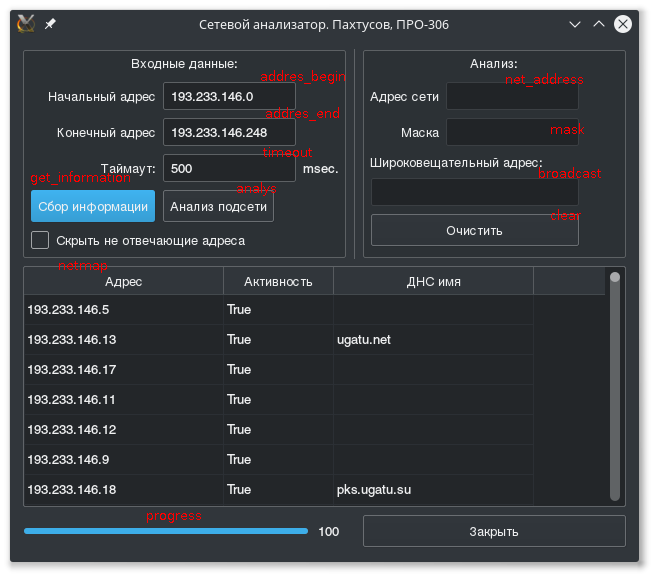
\includegraphics[width=0.8\linewidth]{image10}}
			\caption{Компоненты основного окна.}
		\end{figure}
	
		В программе используются следующие библиотеки:

		\begin{itemize}
			\item
				\texttt{socket} -- библиотека, обеспечивающая высокоуровневый сетевой интерфейс.
			\item
				\texttt{pinging} -- библиотека, реализующая ping с помощью raw-сокетов.
			\item
				\texttt{struct} -- библиотека, осуществляющая преобразование объектов в байтовом представлении.
		\end{itemize}
		
		Программа разделена на три модуля: \textbf{View}, \textbf{Controller} и \textbf{Pinging}. Модули объединяются в одну программу с помощью скрипта \texttt{network\_scanner.py}.
		
		\begin{itemize}
			\item Модуль \textbf{View} используется для вывода графики. Это представление, которое обеспечивает функционирование графического интерфейска.
			\item Модуль \textbf{pinging} предоставляет интерфейс для сбора информации о сети. В нем реализованы функции управления потоками и функция \texttt{pinging.is\_up()}.
			\item Модуль \textbf{Controller} -- контроллер, обеспечивающий связь между View и pinging. Именно к нему обращается View, если необходимо собрать информацию о сети и именно с помощью него pinging передает информацию о хостах.	
		\end{itemize}
		
		Controller реализует паттерн <<Наблюдатель>>. Как только обработан один из адресов, посылается уведомление представлению (модуль View), которое добовляет значения в таблицу.
		
		При нажатии кнопки <<Сбор информации>> вызывается метод \texttt{getNetInfo()}, который просит Controller собрать информацию о сети, вызывая метод \texttt{controller.ping(begin, end)}. После этого Controller генерирует необходимый диапазон адресов и передаёт их модулю pinging с помощью \texttt{pinging.async\_ping()}. pinging создаёт необходимое количество потоков с помощью \texttt{multiprocessing.Process().start()}, в каждом из них вызывая функцию \texttt{pinging.us\_up()}. Эта функция находит информацию о статусе ip и его DNS-имени и складывает её в асинхронную очередь. Controller берёт значения из этой очереди и передаёт их во View с помощью функции \texttt{view.addToATable()}. 
		
		При нажатии кнопки <<Анализ подсети>> вызывается функция View \texttt{subnetAnalys()}. Для анализа сети служит функция \texttt{controller.find\_mask\_net\_addr\_broadcast()}, которую вызывает View. В ней последовательно вызываются функции для определения маски (\texttt{pinging.subnet\_mask}), адреса сети (\texttt{pinging.network\_address}), широковещательного адреса (\texttt{pinging.broadcast\_address}) и адреса шлюза (\texttt{pinging.gateway\_address}). Функция возвращает кортеж с этими значениями. Эти значения View записывает в соответствующие текстовые поля.
		
		\begin{figure}[H]
			\center{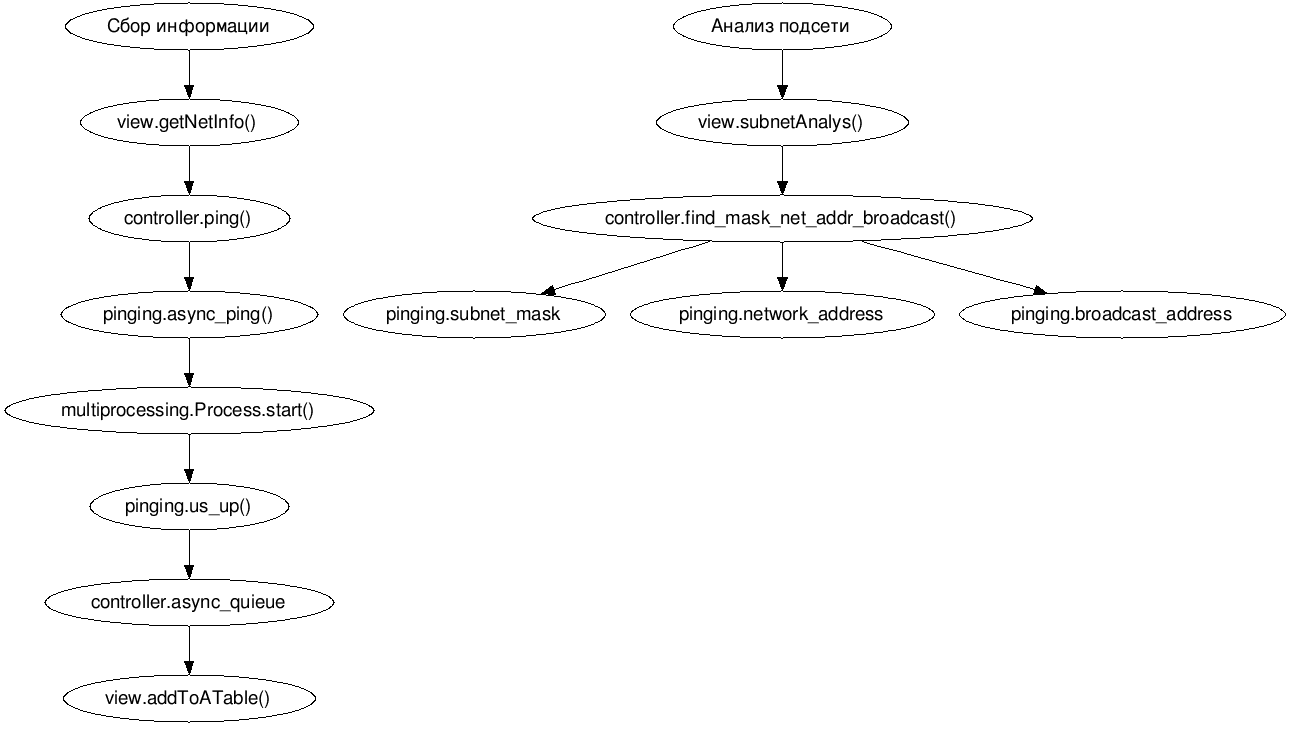
\includegraphics[width=0.8\linewidth]{func_scheme}}
			\caption{Функциональная схема программы}
		\end{figure}
		
		Рассмотрим код, который реализует необходимые функции:
		
		\begin{itemize}
			\item \textbf{Ввод диапазона адресов}. В модуле \texttt{View}:
			
			\begin{verbatim}
def getNetInfo(self):
    ...
    self.address_begin.text()
    self.address_end.text()
    int(self.timeout.text())
    ...
			\end{verbatim}
			
			\item \textbf{Генерация адресов.} В модуле \texttt{Controller}:
			\begin{verbatim}
def ping(self, address_begin, address_end, timeout):
        begin = ipaddress.IPv4Address(address_begin)
        end = ipaddress.IPv4Address(address_end)
        addresses = []
        while begin <= end:
            addresses.append(str(begin))
            begin = begin + 1
            
        ...
			\end{verbatim}
		
			\item \textbf{Реализация многопоточности.} В модуле \texttt{Controller} (для того, чтобы освободить основной поток):
			
			\begin{verbatim}
def ping(self, address_begin, address_end, timeout):
    ...
    p = Process(target=self.async_ping, args=(addresses, timeout))
    p.start()
    ...
			\end{verbatim}
			
			В модуле \texttt{Pinging}:
			
			\begin{verbatim}
def pg(addresses, queue, timeout):
    processes = [
        Process(target=pinging, args=(addr, queue, timeout))
        for addr in addresses
    ]
    n = 20
    processes = [processes[i:i + n] for i in range(0, len(processes), n)]
    for pr in processes:
        for p in pr:
            p.start()
        for p in pr:
            p.join().
			\end{verbatim}	
			
			\item \textbf{Определение работоспособности узла и DNS-имени.} В модуле \texttt{Pinging}:
			
			\begin{verbatim}
def pg(addresses, queue, timeout):
    try:
        up = is_up(addres, timeout)
    except:
        up = False
    name = str()
    if up:
        print(addres)
    try:
        name, _, _ = socket.gethostbyaddr(addres)
        print(name)
    except:
        pass
    queue.put((addres, up, name))
			\end{verbatim}
			\item \textbf{Анализ информации подсети.} В модуле \texttt{Controller}:
			\begin{verbatim}
def find_mask_net_addr_broadcast(self, addresses):
    ...
    mask = net_mod.subnet_mask(addresses) #self.find_mask(addresses)
    subnet = net_mod.network_address(mask, addresses[0])
    broadcast = net_mod.broadcast_address(mask, subnet)
			\end{verbatim}
			
			
			 В модуле \texttt{Pinging}:
			 \begin{verbatim}
def subnet_mask(ip_list):
    def convert_to_bin_str(arg):
        return bin(struct.unpack('>I', socket.inet_aton(arg))[0])[2:]
    ip_list = list(map(convert_to_bin_str, ip_list))
    prefix = os.path.commonprefix(ip_list)
    bm = '1' * len(prefix) + '0' * (32 - len(prefix))
    binary_mask = int.to_bytes(int(bm, 2), 4, byteorder='big')
    return socket.inet_ntoa(binary_mask)
    
def network_address(mask, address):
    mask = struct.unpack('>I', socket.inet_aton(mask))[0]
    address = struct.unpack('>I', socket.inet_aton(address))[0]
    return socket.inet_ntoa(struct.pack('>I', mask & address))
    
def broadcast_address(mask, network):
    mask = '.'.join(list(map(lambda x: str(255-int(x)), mask.split("."))))
    mask = struct.unpack('>I', socket.inet_aton(mask))[0]
    network = struct.unpack('>I', socket.inet_aton(network))[0]
    return socket.inet_ntoa(struct.pack('>I', mask | network))
			\end{verbatim}
			 
			
		\end{itemize}
			
		\subsubsection{Руководство пользователя}

		\begin{figure}[H]
			\center{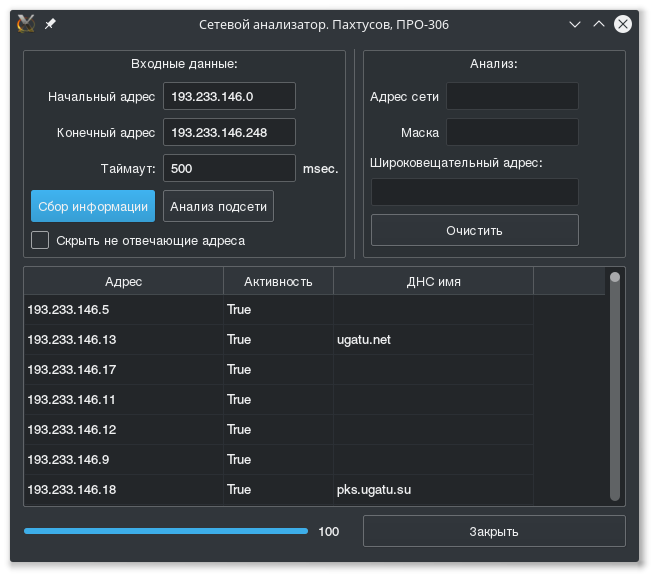
\includegraphics[width=0.8\linewidth]{image11}}
			\caption{Основное окно программы}
		\end{figure}
		
		Для выбора диапазона адресов необходимо установить значения каждого байта адреса с помощью текстовых полей. После установки начального и конечного адресов нужно нажать кнопку <<Сбор информаци>>. В результате заполнится таблица, в которой отражена работоспособность узла, адрес узла и его символьное имя. Индикатор внизу таблицы показывает выполнение обработки.

		Для анализа сети необходимо выделить в таблице адреса, затем нажать на кнопку <<Анализ подсети>>. В результате заполнятся соответствующие текстовые поля с адресом сети, маской сети и широковещательным адресом.
		
		\subsubsection{Результат анализа сети}

Результат анализа сети можно представить в виде таблицы:

\begin{center}
\begin{longtable}{|l|l|}
\hline
Кафедра&Информация о сети\\
\hline
\multirow{4}{*}{Кафедра информатики}&Маска сети: 255.255.255.252\\
&Адрес сети: 193.233.146.32\\
&Широковещательный адрес: 193.233.146.35\\
&Адрес шлюза: 193.233.146.33\\
\hline
\multirow{4}{*}{Кафедра ВТИЗИ}&Маска сети: 255.255.255.248\\
&Адрес сети: 193.233.146.40\\
&Широковещательный адрес: 193.233.146.47\\
&Адрес шлюза: 193.233.146.41\\
\hline
\multirow{4}{*}{Кафедра АД}&Маска сети: 255.255.255.252\\
&Адрес сети: 193.233.146.48\\
&Широковещательный адрес: 193.233.146.51\\
&Адрес шлюза: 193.233.146.49\\
\hline
\multirow{4}{*}{Кафедра математики}&Маска сети: 255.255.255.252\\
&Адрес сети: 193.233.146.72\\
&Широковещательный адрес: 193.233.146.75\\
&Адрес шлюза: 193.233.146.73\\
\hline
\multirow{4}{*}{Кафедра ГИС}&Маска сети: 255.255.255.252\\
&Адрес сети: 193.233.146.76\\
&Широковещательный адрес: 193.233.146.79\\
&Адрес шлюза: 193.233.146.77\\
\hline
\multirow{4}{*}{Кафедра ТКС}&Маска сети: 255.255.255.252\\
&Адрес сети: 193.233.146.80\\
&Широковещательный адрес: 193.233.146.83\\
&Адрес шлюза: 193.233.146.81\\
\hline
\multirow{4}{*}{Кафедра ТС}&Маска сети: 255.255.255.248\\
&Адрес сети: 193.233.146.224\\
&Широковещательный адрес: 193.233.146.231\\
&Адрес шлюза: 193.233.146.225\\
\hline
\multirow{4}{*}{Кафедра АСУ}&Маска сети: 255.255.255.248\\
&Адрес сети: 193.233.146.232\\
&Широковещательный адрес: 193.233.146.239\\
&Адрес шлюза: 193.233.146.233\\
\hline
\multirow{4}{*}{Кафедра ВМК}&Маска сети: 255.255.255.248\\
&Адрес сети: 193.233.146.240\\
&Широковещательный адрес: 193.233.146.247\\
&Адрес шлюза: 193.233.146.241\\
\hline
\multirow{4}{*}{Кафедра ТОЭ}&Маска сети: 255.255.255.252\\
&Адрес сети: 193.233.146.248\\
&Широковещательный адрес: 193.233.146.251\\
&Адрес шлюза: 193.233.146.249\\
\hline
\end{longtable}
\end{center}

\subsubsection{Карта сети}

\begin{figure}[H]
\center{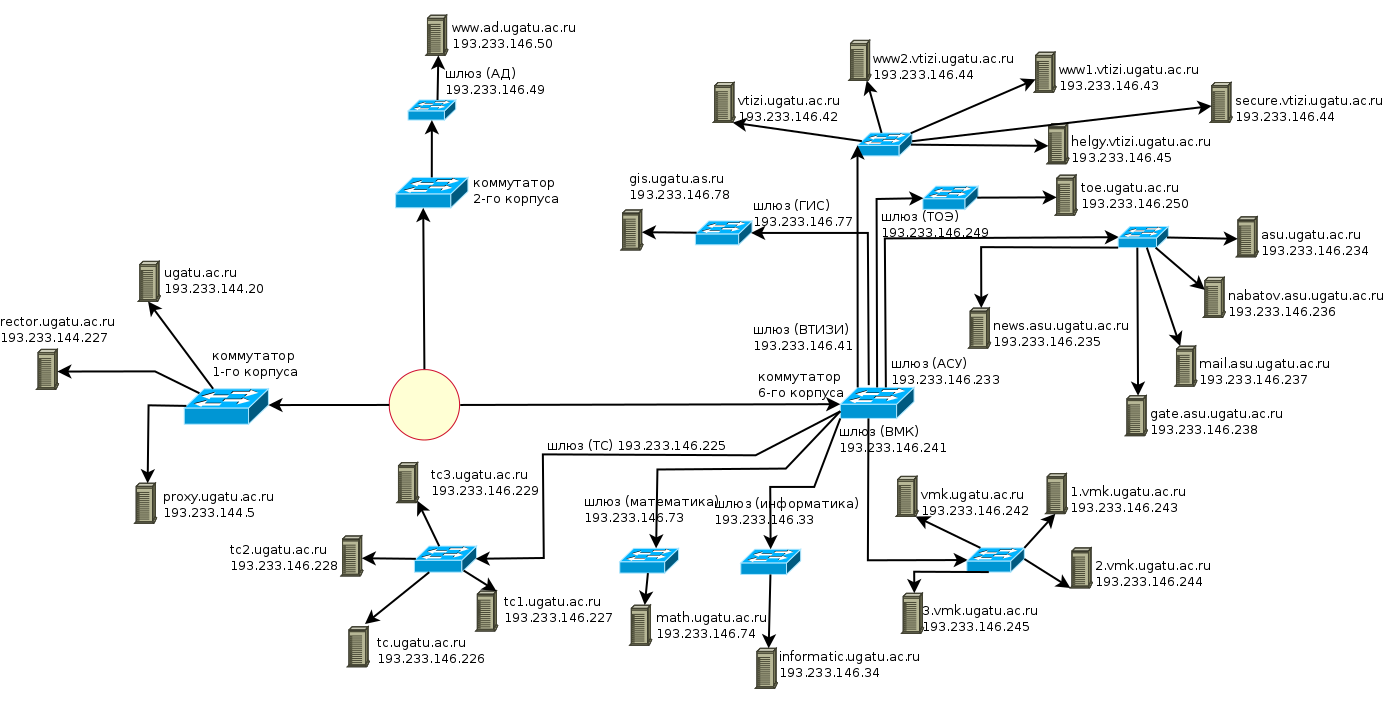
\includegraphics[angle=90,width=0.6\linewidth]{dia_map}}
\caption{Карта сети}
\end{figure}
\FloatBarrier

\section{Заключение}

В результате выполнения данной лабораторной работы были получены знания о настройке TCP/IP параметров компьютера, были получены знания о конфигурировании межсетевого экрана и было написано приложение для сбора информации о сети и её анализе.





		
\end{document}
